The following chapter presents well-established theory on the efficient market hypothesis, before addressing deep learning and neural networks. Lastly, theory on trading strategies are presented, and how deep learning algorithms can be implemented.

\section{The Efficient Market Hypothesis}
The efficient market hypothesis is an economic theory introduced a generation ago, which was widely accepted among financial academics. A general view is that markets are extremely efficient in terms of reflecting news and new information in stock prices without delay. The efficient market hypothesis represents the idea of a "random walk", where in a price series, all subsequent price changes have random departures from previous prices. Information and news is believed to be immediately reflected in stock prices, which means that future stock price changes reflect only future news and is therefore independent of previous price changes. In other words, there is no correlation between tomorrow's price change and today's price change. New information regarding a stock is considered to be unpredictable, meaning that price changes are also unpredictable and random. Thus, stock price predictions based on either technical or fundamental analysis does not enable an investor to earn excess returns without accepting excess risk \cite{malkiel}. 

\indent \newline 
The hypothesis is commonly interpreted in three forms, which consist of a weak, semi-strong and strong form of efficiency. The weak form represents a market efficiency where prices reflect previous historical prices and returns. This implies that an investor is not able to use technical analysis as a method for earning excess returns. Semi-strong form of efficiency consists of prices reflecting publicly available information, e.g. quarterly reports, stock splits, issue of shares, etc. This implies that an investor is not able to make use of fundamental analysis to earn excess returns. Finally, a strong form of efficiency represents prices where all information related to a stock, including information only available to company insiders, is reflected \cite{fama}. 

\indent \newline 
Jensen's Alpha ($\alpha$) is a term within finance which was introduced in the late 1960's by Michael Jensen. The term is a post-hoc metric which evaluates a portfolio's ability to earn above-average returns adjusted for market risk. A positive Alpha means that the portfolio is able to generate a higher rate of return than the market as a whole, or some sort of benchmark index, while a negative Alpha translates to an underperforming portfolio compared to the market rate of return \cite{inproceedings}. Opposed to the more general term Alpha, Jensen's Alpha takes into consideration the capital asset pricing model (CAPM) market theory and adjusts for risk in its calculations. The formula for Jensen's Alpha is as follows:

\indent \newline 
\textit{Jensen’s Alpha = Portfolio Rate of Return - Benchmark Portfolio Rate of Return}

\indent \newline 
\textit{Benchmark Portfolio Rate of Return = R_{f} + $\beta$ (R_{m} - R_{f})}

\indent \newline 
\textit{Where,
\begin{itemize}
    \item[] $R_{f}$ = Risk Free Rate of Return
    \item[] $\beta$ = Beta
    \item[] $R_{m}$ = Expected Market Return
\end{itemize}
}

\indent \newline 
The risk free rate of return is a representation of an investment with zero risk. A common way to find the correct risk free rate of return is to subtract the inflation rate from the yield of a treasury bond, which matches the investment duration. The U.S. treasury bill is an often used measure for a risk-free rate since the broad market considers there to be zero probability of the government defaulting on their obligations \cite{chen1}. Beta is a measure of a portfolio's systematic risk, which represents the risk component that an investor is not able to avoid. It is used for measuring a stock's volatility and how much it fluctuates relatively to the rest of the market \cite{Kenton}. Beta can be found through the following calculation:

\[Beta = \frac {Covariance(R_{e},R_{m})}{Variance(R_{m})}\]

\indent \newline 
\textit{Where,
\begin{itemize}
    \item[] $R_{e}$ = The return on an individual stock
    \item[] $R_{m}$ = The return on the overall market
    \item[] $Covariance$ = How changes in a stock's returns are related to changes in the market's return
    \item[] $Variance$ = How far the market's data points spread out from their average value
\end{itemize}
}

\indent \newline 
From an investor's point of view, the key points of the efficient market hypothesis suggest that it is not possible to generate consistent alpha, and therefore no point of actively managing a portfolio. This means that a portfolio manager is not able to earn excess returns through the use of technical analysis nor fundamental analysis. 

\indent \newline 
Previous research has presented evidence both for and against the efficient market hypothesis. In 1978, Michael C. Jensen argued that there was no other proposition in economics with more supportive, empirical evidence than the efficient market hypothesis \cite{JENSEN}. However, in the article he acknowledged that times were moving forwards with better data- and econometric analysis which uncovered anomalies and inconsistency with previous evidence supporting the hypothesis. Further, in 1980 Grossman and Stiglitz addressed the issue of prices fully reflecting all available information. They argued that prices only partially reflect available information, where those who obtain information are adequately compensated  \cite{stiglitz}. If prices reflected all information, then there would be no financial incentive to obtain information. This would affect the market efficiency in terms of there not being arbitrators in the market, who have a function of keeping the market efficient.

\indent \newline 
The strong form of the efficient market hypothesis was corrected by Fama in 1991, which was previously based on the assumption of zero costs associated with obtaining information and carrying out transactions. It was assumed that only if transaction costs and costs of obtaining information were equal to zero, investors would have the incentive to keep trading until prices reflected all available information. In reality these costs are positive (greater than zero), which does not correspond with the previous assumption. Fama redefined this part of the strong form of market efficiency as stock prices reflecting available information until the marginal usefulness of information is equal to the marginal cost \cite{lekovic}. A few years later, Fama addressed the issues with anomalies and referred to them as a result of chance. With an expected value of above-average return of zero, anomalies in the form of under- and overreactions are due to chance. Fama also believed anomalies to be a result of incorrect methodology \cite{lekovic}.

\indent \newline 
Being that there does not exist conclusive evidence either for or against the efficient market hypothesis, the aim of the paper is to test if the weak-form of the efficient market hypothesis holds or not. The hypothesis will be implicitly tested in terms of examining if it is possible to achieve above-average returns using deep learning-models that are based on technical analysis, and also if the application of deep learning differs between small cap- and large cap stocks.   

\section{Mean Reversion}
Mean reversion is a financial theory where supporters of the theory believe that a stock's historical returns and price volatility will eventually revert to the long-term mean, or the mean for the entire dataset \cite{chenj}. Investors who base their investing strategy on this theory try to utilize the fluctuations in stock prices, with an expectation of the price eventually converging to the average price over time. Thus, if a stock price drops abnormally low, the theory suggests that it is probably a good time to buy, while if a stock rises abnormally high it is most likely time to sell, or perhaps even go short. The theory relates to the idea of buying low and selling high, which is a strategy that can be applied to most securities. However, there is no guarantee that a stock price will converge to the average price level. Several changes could happen which can affect the future outlook of a stock, both at a company level, market segment level, or the market as a whole. This applies to both a more positive and negative outlook for the company, which can be exemplified by a new breakthrough technology or a pending lawsuit. 

\indent \newline 
James M. Poterba conducted research on the topic in 1988 with his article titled "Mean reversion in stock prices: Evidence and Implications" \cite{poterba}. In the article he states that "if market and fundamental values diverge, but beyond some range the differences are eliminated by speculative forces, then stock prices will revert to their mean". Hence, if the market value exceeds a threshold where the price reaches a level which can not be explained by fundamental values, the price will start converging to the mean. When stocks are incorrectly priced and eventually reverted to the mean, returns need to be negatively serial correlated at some frequency. The resulting findings from the research showed a positive serial correlation in stock returns over short periods and negative correlation over longer time periods. The statistical tests could not consistently reject the random-walk hypothesis at high significant levels, but at an aggregated level the evidence pointed to transitory components having a high explanatory effect on the variance in returns.    

\indent \newline 
The findings related to mean reversion could potentially strengthen the assumption of deep learning algorithms being able to find patterns within historical data. Based on the theory, including securities' moving averages should enable neural networks to make predictions of profitable entry- and exit price levels.  

\section{Technical Analysis}
As mentioned in the previous section, technical analysis is an investing technique that contradicts the weak form of the efficient market hypothesis. The investing strategy is a tool which tries to predict future price movements based on historical prices and other technical indicators like trends, volume, moving averages, support- and resistance levels, and momentum. While long-term investors focus more on time spent in the market, investors who use technical analysis are more focused on timing the market. The tool is used for timing profitable entry- and exit points, and it usually consists of more frequent trading.   

\indent \newline 
Investtech is a Norwegian company which specializes in behavioral finance and technical analysis of stocks. They offer stock analysis based on advanced mathematical models and statistical optimization. The analyses are a result from more than 20 years of research on stocks that are listed on the Nordic stock exchanges. Their research shows supporting evidence of the ability to achieve above-average returns using technical analysis. Some of the resulting findings on various technical indicators include:

\begin{itemize}
  \item \textbf{Rising trend} - stocks that are in a rising trend channel yield annual excess returns of 7.8\% in the medium long term.
\begin{figure}[H]
\centering
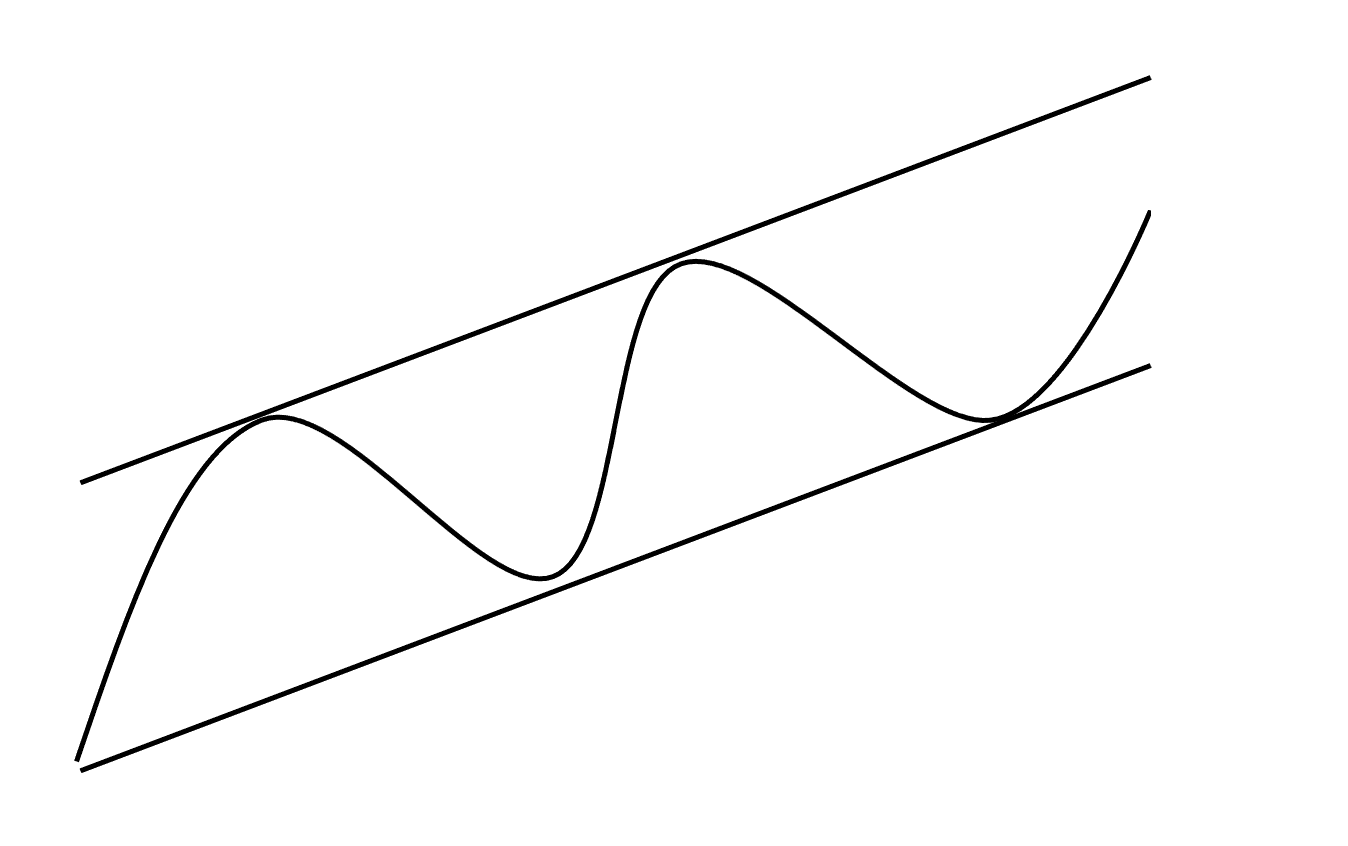
\includegraphics [scale=0.20,angle=360]{figures/trendup.png}
%\caption{Illustration of a Neural Network}
\label{fig:trendup}
\end{figure}
  \item \textbf{Falling trend} - stocks that are in a falling trend channel yield annual below-average returns of 11.4\% in the medium long term.
\begin{figure}[H]
\centering
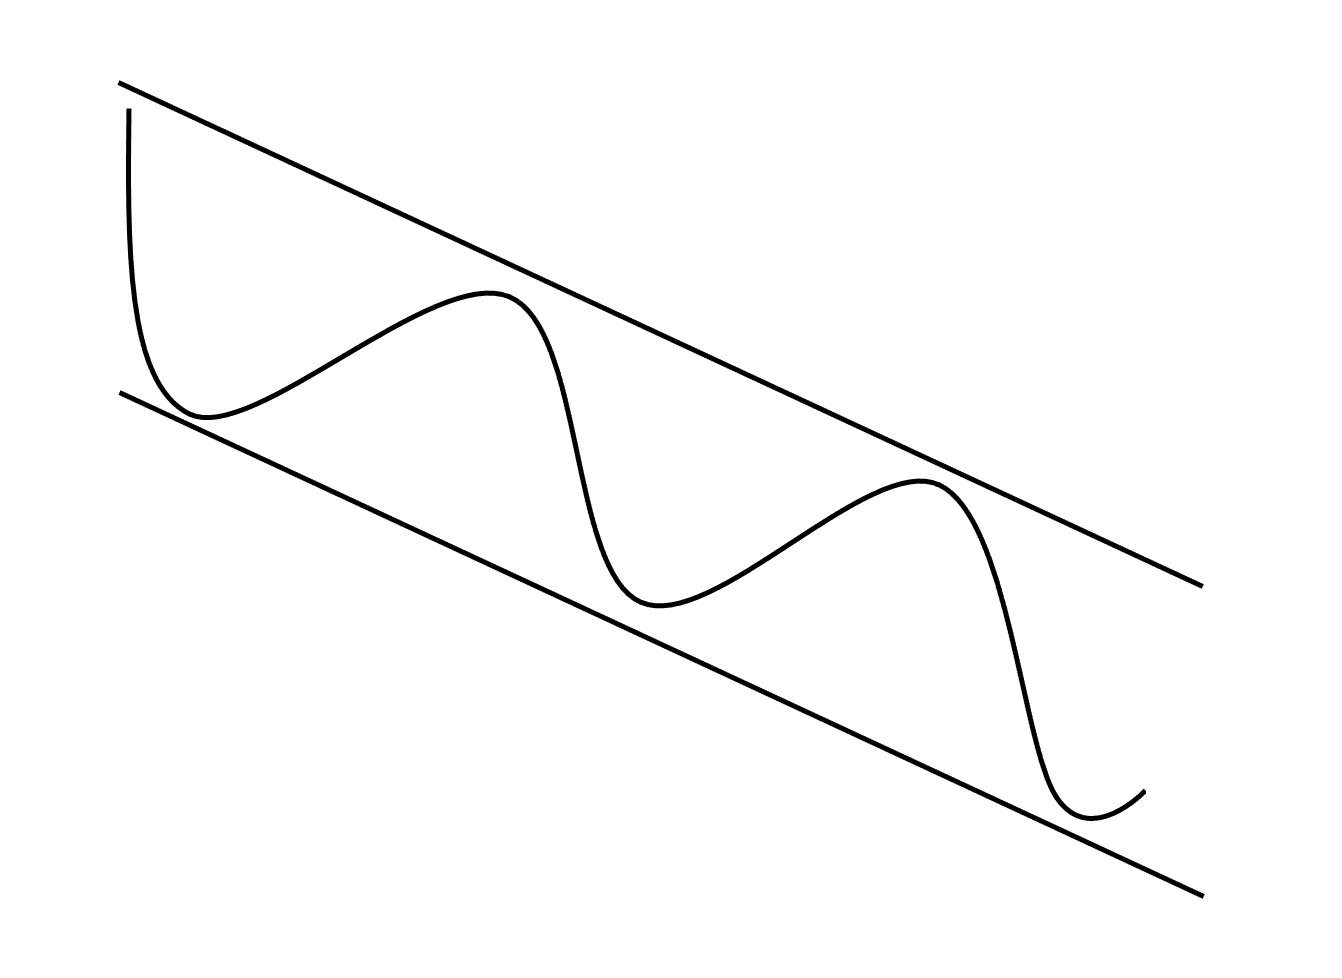
\includegraphics [scale=0.20,angle=360]{figures/trenddown.png}
%\caption{Illustration of a Neural Network}
\label{fig:trenddown}
\end{figure}
  \item \textbf{Trend break up} - stocks in rising trend channels which break up through the ceiling of the channel yield 14.7\% in annual excess returns in the medium long term.
\begin{figure}[H]
\centering
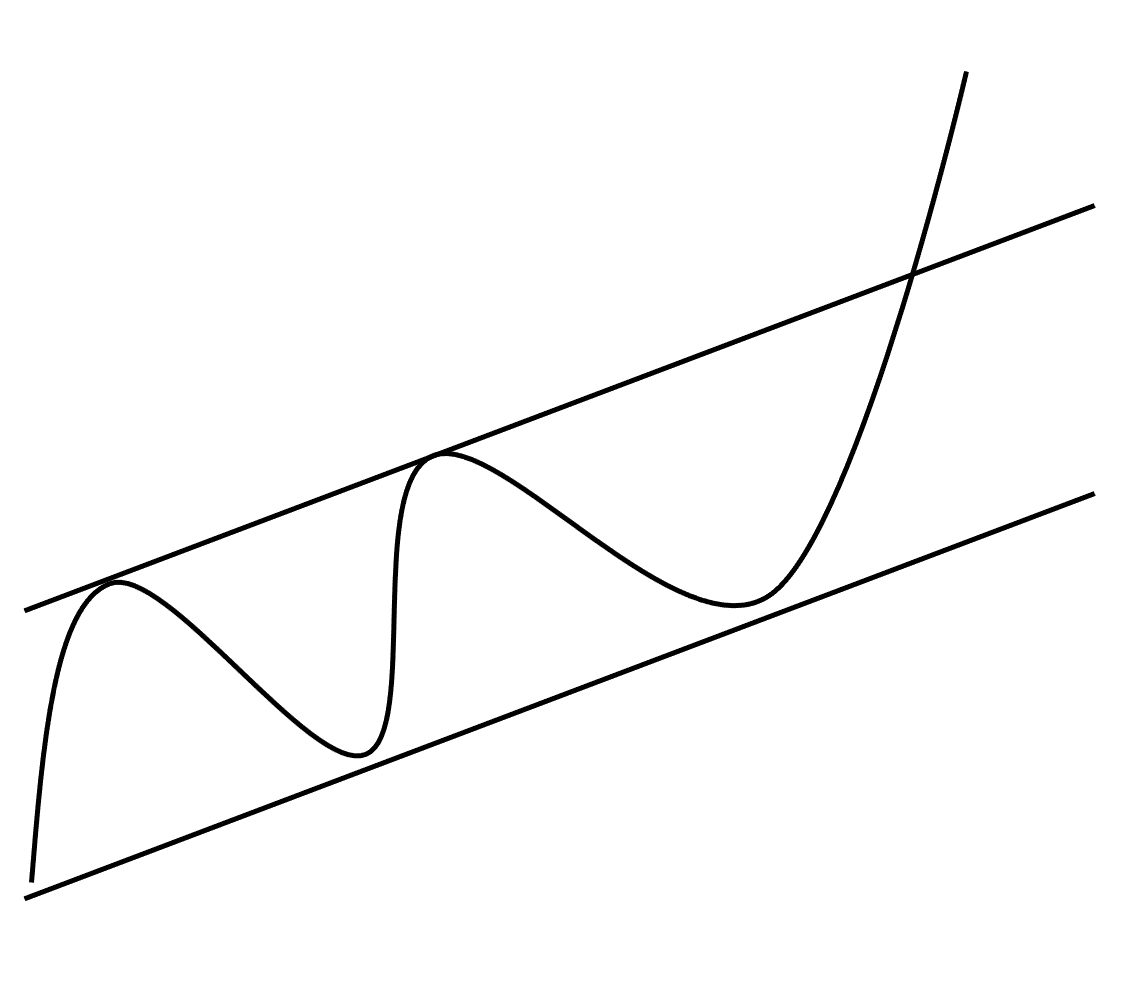
\includegraphics [scale=0.20,angle=360]{figures/breakup.png}
%\caption{Illustration of a Neural Network}
\label{fig:breakup}
\end{figure}
  \item \textbf{Trend break down} - stocks in falling trend channels which break down through the channel floor yield 27.9\% in annual below-average returns in the medium long term.
\begin{figure}[H]
\centering
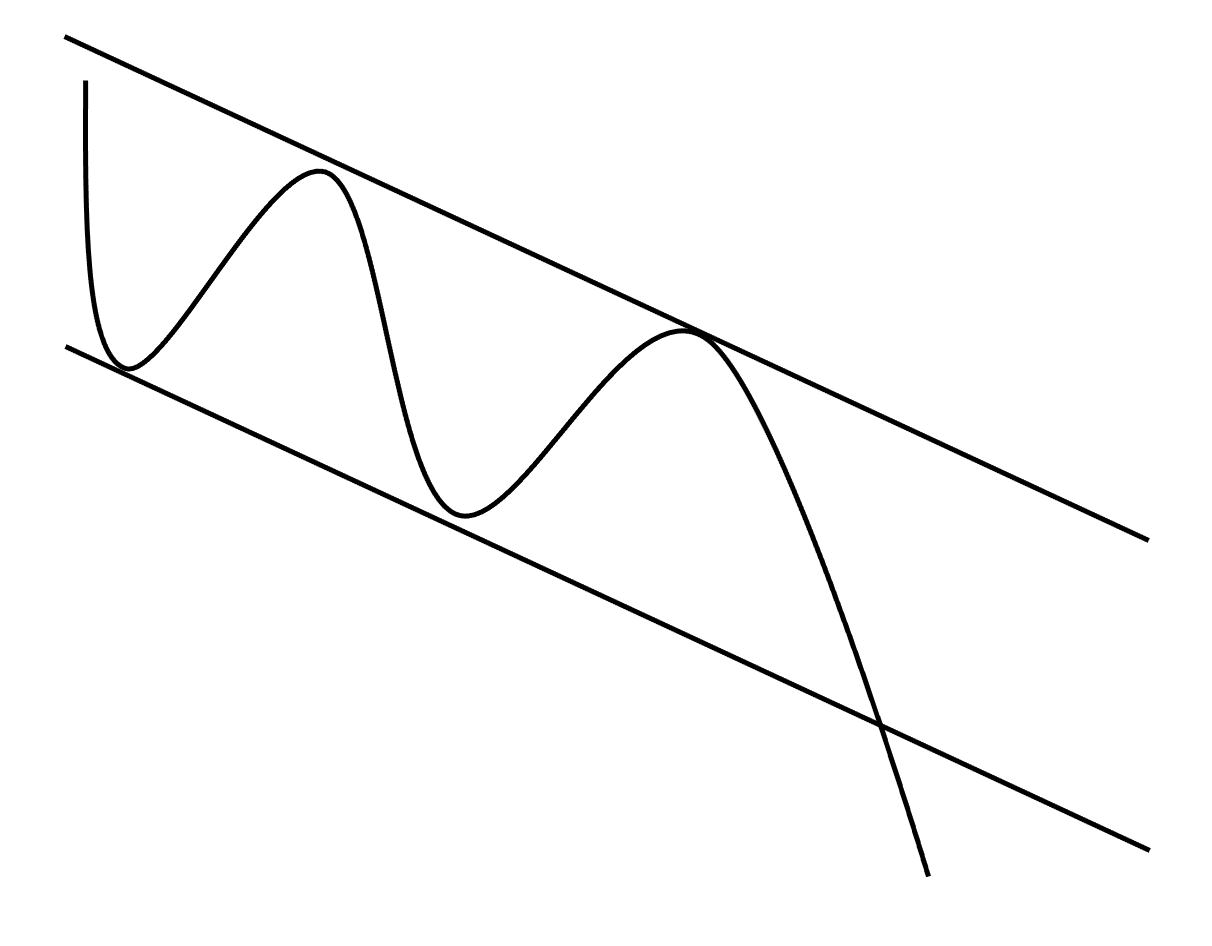
\includegraphics [scale=0.20,angle=360]{figures/breakdown.png}
%\caption{Illustration of a Neural Network}
\label{fig:breakdown}
\end{figure}
  \item \textbf{Positive volume balance} - stocks with a positive volume balance yield annual excess returns of 4.7\% in the medium long term.
\begin{figure}[H]
\centering
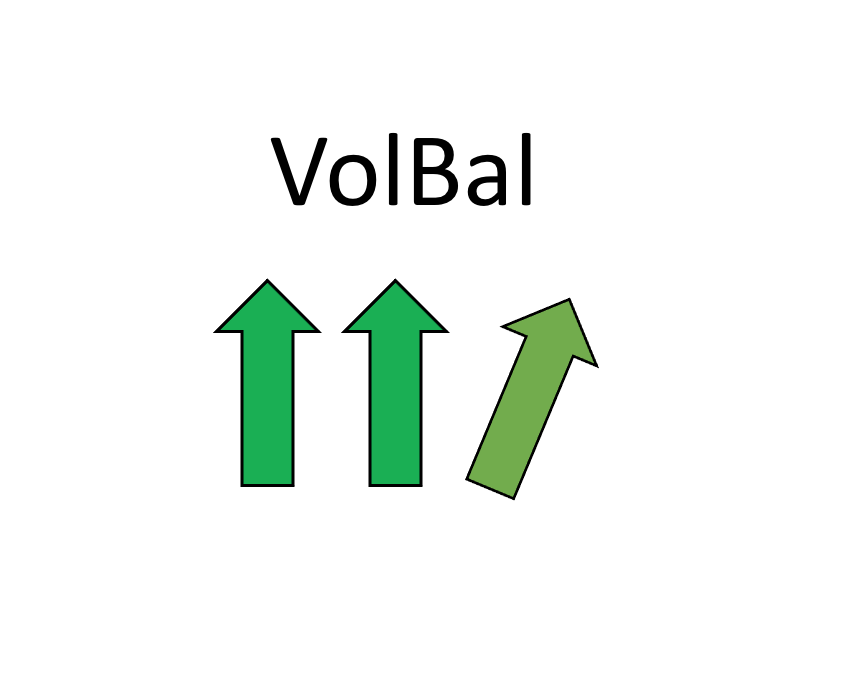
\includegraphics [scale=0.20,angle=360]{figures/volumepos.png}
%\caption{Illustration of a Neural Network}
\label{fig:volumepos}
\end{figure}
  \item \textbf{Negative volume balance} -  stocks with a negative volume balance yield annual below-average returns of 7.6\% in the medium long term.
\begin{figure}[H]
\centering
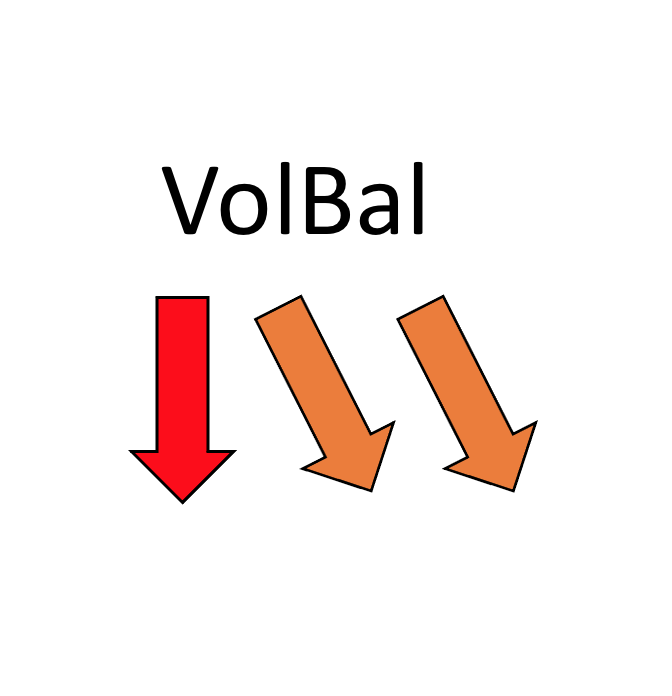
\includegraphics [scale=0.20,angle=360]{figures/volneg.png}
%\caption{Illustration of a Neural Network}
\label{fig:volneg}
\end{figure}
  \item \textbf{Strong positive momentum} - stocks with strong positive momentum yield 11.4\% in annual excess returns in the medium long term.
\begin{figure}[H]
\centering
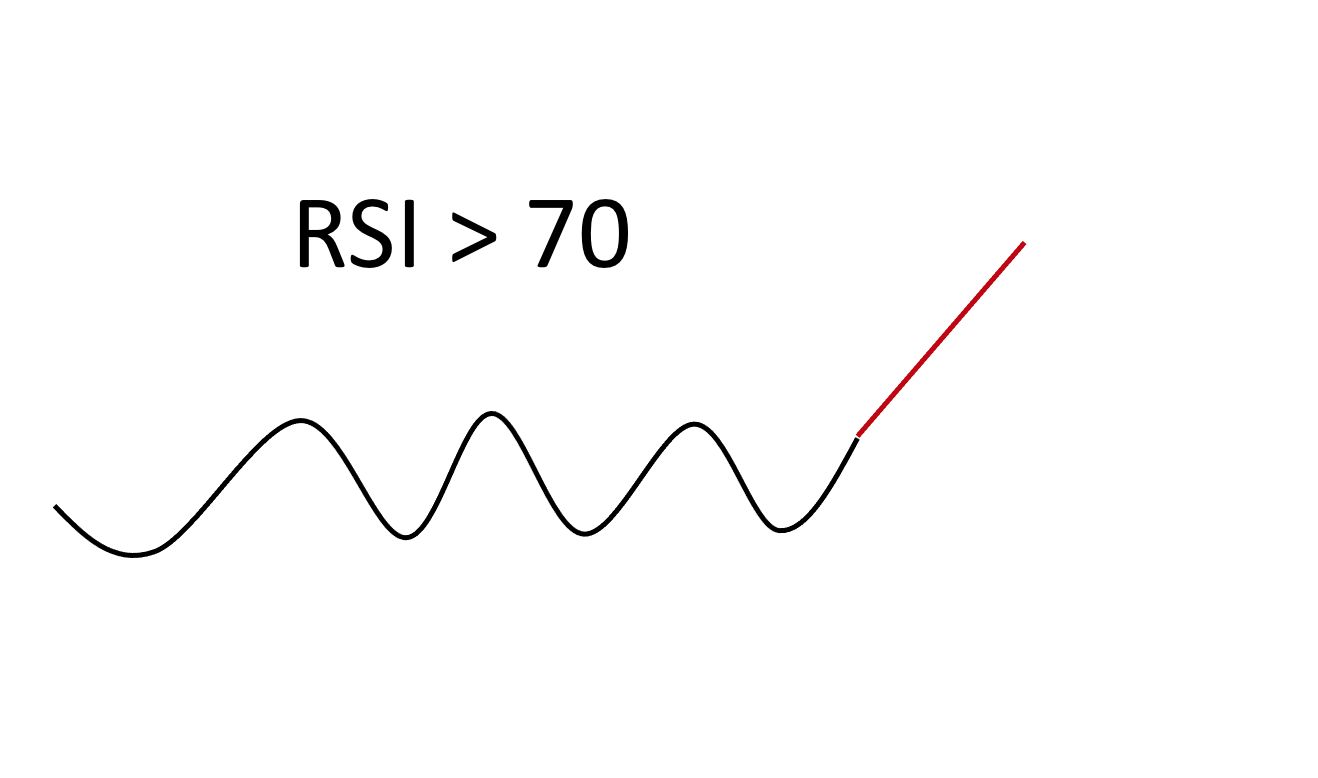
\includegraphics [scale=0.20,angle=360]{figures/momentumpos.png}
%\caption{Illustration of a Neural Network}
\label{fig:momentumpos}
\end{figure}
  \item \textbf{Strong negative momentum} - stocks with strong negative momentum yield 13.3\% in annual below-average returns in the medium long term. 
\begin{figure}[H]
\centering
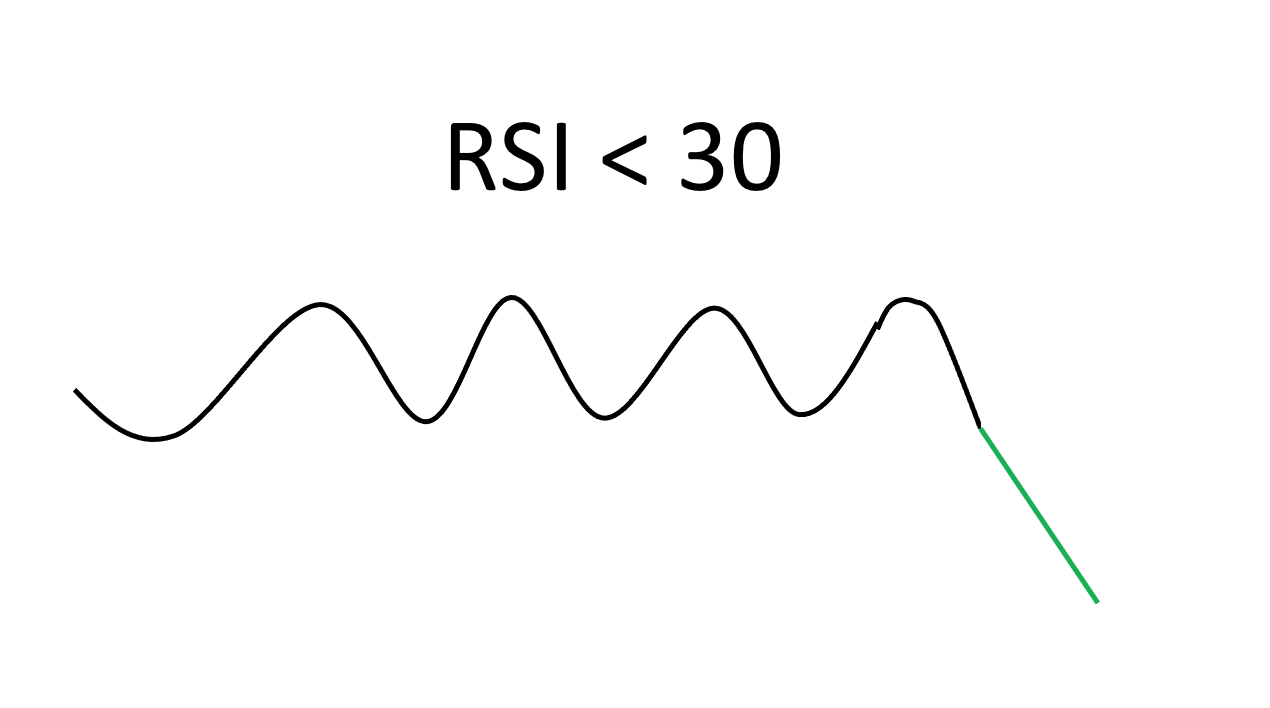
\includegraphics [scale=0.20,angle=360]{figures/momneg.png}
%\caption{Illustration of a Neural Network}
\label{fig:momneg}
\end{figure}  
\end{itemize}
\indent \newline 
\cite{investtech}

\indent \newline 
There are numerous different indicators and measures within the field of technical analysis, and the importance of each one varies greatly between investors. However, the main object of this type of investing strategy is to capture both the market psychology as a whole and also for individual stocks. Investors who utilize technical analysis seek to identify levels of a stock price where there are likely more buyers than sellers (will often lead to an increase in price) and levels where there are likely more sellers than buyers (will often lead to a decrease in price). A simplified explanation of the directional movements in price consists therefore of stock prices being greatly dependent on supply and demand. The level of aggressiveness among buyers and sellers is another factor which affects the movements of a stock price, and captures the psychological state of mind of the investors. Sellers who close their position by aggressively selling at bid, represent a situation where there is little optimism among investors and a probable decline in short-term price. Buyers who open positions by aggressively buying at ask, represents a situation where there is a lot of optimism among the investors and anticipations of a short-term increase in the stock price. 

\indent \newline 
Investors (traders) who base their investing strategy on technical analysis believe that the market psychology can be found in historical charts, prices and other technical measures, and that history repeats itself. An example of this is if a stock has previously reversed when falling to a certain price level on multiple occasions, the chances are that this will happen again. This is called a support level and represents a situation where there are many investors who believe the stock is cheap, and few sellers because they feel the stock is undervalued. Hence, there is a high probability that the stock price will increase based on a revitalized optimism among the investors again. This is under the assumption that there has not been any fundamental news that changes the company's future outlook.    

\indent \newline 
In order for technical analysis to work as either an investing strategy or investing tool, there must exist patterns within historical data that can be taken advantage of. If investors, through the use of technical analysis, are able to achieve above-average returns, it means that there must exist certain inefficiencies and that the weak form of the efficient market hypothesis does not hold. Instead of manually having to search for and detect these inefficiencies, this paper aims to utilize deep learning algorithms as an automated substitute for finding patterns within the data, representing potentially valuable entry points and ultimately above-average returns. Theory on deep learning is explained in the next section.          


\section{Machine Learning}
Modern enterprises today utilize the power of machine learning and computational power to assist every day-operations and operational decisions. Implementing analytics as an automated decision tool throughout the entire organization was previously characterized by tech-companies like Google, Amazon, Facebook etc, but in recent years this trend has changed. More and more mainstream companies are trying to replicate the success of these tech-companies by developing predictive models, visualization models, and other types of data-driven models to support operational decisions. Even though analytics and machine learning just recently has started to be recognized as a business asset, and not just a separate business project, the concepts of machine learning have been around for many years.  

\subsection{History}
Machine learning is partly based on the brain cell interaction-model created in 1949 by Donald Hebb in the book titled "The Organization of Behaviour". Hebb presented theories on neuron excitement and communication between neurons, which can be translated into the concepts of artificial neural networks and artificial neurons \cite{dataversity}. In the 1950’s Arthur Samuel came up with the phrase "Machine Learning". He developed a chess computer program based on alpha-beta pruning, where the program chooses the next move by using a minimax strategy and a scoring function. Samuel introduced rote learning, where the program recorded all previous positions and combined this with the reward function. In the same decade, Frank Rosenblatt built upon the work of Hebb and Samuel by creating the perceptron. The program was designed for image recognition. However, the program did not produce satisfying results, where it was only able to recognize a few kinds of visual patterns. This led to a stagnation in the research of machine learning and neural networks, which lasted until the 1990's. 

\indent\newline
In 1967, Marcello Pelillo was given credit for developing the nearest neighbour algorithm. The algorithm was developed in connection with the traveling salesperson's problem, where the algorithm was used for mapping routes and finding the most efficient one. This is considered as the beginning of basic pattern recognition. Further in the same decade, multilayers were introduced in the research of neural networks. Using more than one layer in the perceptron resulted in a significant increase in processing power, which laid the foundation for the future development of feedforward neural networks and backpropagation. The backpropagation algorithm differs from feedforward neural networks by having the ability to process output errors and distribute them backwards through the layers of the network. This improves the learning ability of the network and is currently being used to train deep neural networks \cite{dataversity}. 

\indent\newline
During the period from the 1970's and 1990's the fields of machine learning and artificial intelligence were separated. Machine learning had previously been incorporated as a training program for artificial intelligence, but shifted focus to solve more service-oriented tasks during this period. Machine learning flourished in the 1990's as a result of the internet growth and focus on neural networks. Increased access to digital data and an easier ability to share data and services was the main reasoning behind the revived success of machine learning during this decade. In this decade, Robert Schapire introduced the concept of boosting. This is a technique developed to reduce bias during supervised learning and to transform weak learners into strong learners. Boosting algorithms create a final strong classifier by repetitive learning weak classifiers. Each weak classifier is weighted based on the learner’s accuracy and then reweighted. The weight of misclassified input data increases, while the weight of correctly classified data decreases, in order for future weak learners to focus more on previous misclassified weak learners. Strong learners are easily classified aligned with the true classification, while weak learners are only slightly correlated with the true classification \cite{dataversity}. 

\indent\newline
Ever since the millennium, machine learning has been applied to several business areas. In the early 2000's, speech and facial recognition technology was developed. Speech recognition is based on Long Short-Term Memory (LSTM), which is a neural network technique developed by Jürgen Schmidhuber and Sepp Hochtreiter in 1997. LSTM is particularly relevant for speech recognition in terms of being able to learn tasks that require the model to be able to memorize discrete steps that took place thousands of steps earlier. The relevance of the model was highlighted in 2015 when Google's speech recognition program gained a 49\% increase in performance by using a LSTM model. During the same period, newly developed facial recognition algorithms were found to be 10 times more accurate than algorithms from 2002 and 100 times more accurate compared to algorithms applied in 1995 \cite{dataversity}.    

\indent\newline
Today, machine learning is considered as the computer's ability of making automated actions without being explicitly programmed. The applicability of machine learning is relevant for several business areas, which include:
\indent \newline
\begin{itemize}
\item {\textbf{Self-driving vehicles} - Autonomous cars are currently being developed with the use of machine learning and deep learning. These cars have the ability to steer, accelerate and brake, based on prior knowledge, stimuli and past experiences. Prior knowledge includes street maps, the meaning of signs, what to stop for etc. Stimuli are made up of a combination of sensors like vision, lidar, radar, GPS and voice commands, while past experiences can for example be how braking and steering affects direction and speed.  where prior knowledge like street maps, meaning of signs, what to stop for etc.}
\item {\textbf{Business decisions} - Machine learning is increasingly being used for operational decisions, which covers various business operations like predicting production metrics, the number of new customers based on marketing campaigns, or predicting inventory based on customer demand.}
\item {\textbf{Fraud detection} -Fraud related to tax evasion, money laundering and insurance are common problems for most countries, and cost governments billions of dollars each year. By implementing machine learning and predictive models, governments are now able to prevent and detect fraud in a much more efficient way.}
\item {\textbf{Natural language processing} - Machine learning enables Email filtering, where algorithms are able to detect spam and recognize different categories the Email belongs to. Other examples of natural language processing include smart assistants, improvement in search results where search engines are able to give relevant results based on similar search behaviour, and predictive text like autocorrect and autocomplete.}
\end{itemize}

\indent\newline
Within finance, there is an increasing amount of hedge funds that are utilizing machine learning to get an edge over the broad market. Hedge funds use it as support to anticipate market movements and detect market trends at an early stage. Machine learning models also help them get a better understanding of how specific news will affect the market direction and intensity. The main point by incorporating machine learning in this field is to be able to extract information out of large amounts of data. This can for example be to use satellite data to determine customer traffic in retail or to calculate the level of crude oil storage, or to use natural language processing to analyze market sentiment through large amounts of text related to important macroeconomic factors.    

\section{Deep Learning}
In the field of artificial intelligence, deep learning is a subset of machine learning where neural networks can identify patterns within training data, where they eventually are able to make predictions from new, unseen data. The structure of deep learning is based on the workings of a human brain, where the brain is used to recognize patterns and classify various types of information. Neural networks can be trained to perform several tasks, which include regression, classification and clustering \cite{opper}. Before going more into detail on the network structure and how the network learns, it is important to get an idea of how the human brain functions, which in turn can give a better understanding of how deep learning networks work in practice.

\subsection{Biological Neural Networks}
Artificial neural networks can be compared to biological neural networks in terms of artificial neural networks trying to simulate some of the functionalities of the neural networks in the human brain. The processes are quite similar, where artificial neural networks try to imitate the human brain's biological neurons, but in a more simplified way.  

\indent\newline
\begin{figure}[H]
\centering
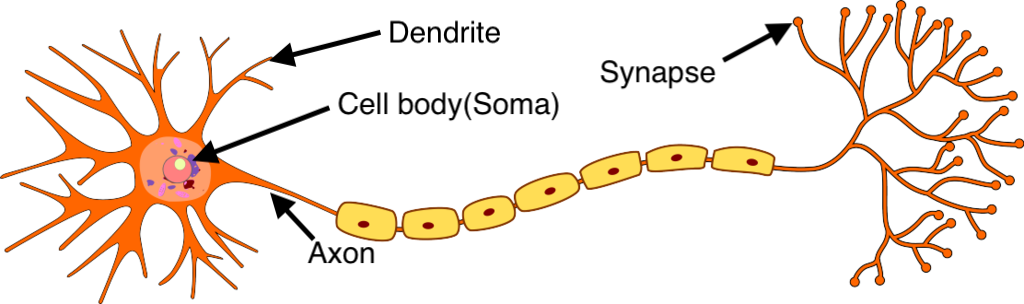
\includegraphics [scale=0.34,angle=360]{figures/bio.png}
\caption{Illustration of a Neuron (source: Wikimedia Commons)}
\label{fig:bio}
\end{figure}
 
\indent\newline   
The figure above illustrates the workings of a nerve cell (neuron) in the human brain. The neurons are arranged together to form a network of nerves, where they transmit and process information received from human senses. These are electrical impulses being passed from one neuron to another. Impulses from the synapse of an adjoining neuron are received through the part of the neuron termed dendrites. The impulses are then carried further to the nucleus (soma), where the electrical impulses are processed before being passed to the axon. The axon consists of a longer branch with a main function of carrying the electrical signal from the soma to the synapse. Lastly, the signal is passed to a neighboring neuron's dendrites, which creates an intricate network of neurons in the human brain \cite{panchal}.  The neurons are electrically excitable due to their membranes' maintenance of voltage gradients. A large amount of change in voltage, in a short amount of time, creates an action potential (electrical pulse) that travels rapidly through the axon and activates adjoining neuron's synaptic connections \cite{opper}.    

\subsection{Neural Network Structure}
As with linear regression, the data consist of independent variables \textit{$x_{n}$}, with an assumption that these features are able to explain the variability in the dependent variable \textit{y}. The target variable can either be continuous or categorical, depending on whether the network is a regression or classification model. Categorical dependent variables consist of a finite number of categories or groups. Examples of a classification model could be predicting gender, type of animals, if an email is spam or not, or classifying customer churn based on recent behaviour. Classification models normally consists of four types of classification, which include:

\begin{itemize}
\item {Binary classification} - This is a very common classification task consisting of having two class labels, where one class represents the normal state and the other class the abnormal state. The class representing the normal state is assigned the value 0, while the class representing the abnormal state is assigned the value 1. Binary classification models usually include a discrete probability distribution, where the models predict the probability of an observation belonging to the two classes.
\item {Multi-class classification} - This type of classification refers to tasks where there are more than two class labels. This means that there could be thousands of known classes, as for example would be the case in face recognition. Normally, a multinoulli probability distribution is incorporated in the predictive model, where the model predicts the probability of an observation belonging to each of the several class labels.
\item {Multi-label classification} - In this case, there are at least two class labels, where the classification task may require predicting more than one class label for each observation. This might be the case in photo classification, where there could potentially be several objects (class labels) in one photo (observation). Also in this type of classification task, it is common to incorporate a discrete probability distribution, where the model predicts multiple outputs and multiple binary classification predictions for each observation.
\item {Imbalanced classification} - The last type of the most common classification problems is imbalanced classification. This type of classification refers to tasks where the number of observations in each class are unequally distributed and where most of the observations belong to the normal class label. A common technique to solve these types of problems consists of combining a normal binary classification model with either undersampling the majority class or oversampling the minority class.
\end{itemize}
\cite{brownlee} 

\indent\newline
Continuous dependent variables have infinite numeric values, which can also consist of date or time. Examples of regression (continuous output) could be predicting next month's sales, traveling time for a specific route, or the number of new customers based on a marketing campaign. In linear regression, coefficients for the independent variables are estimated to make predictions for the target variable, while neural networks incorporate non-linearity and a more intricate structure to gain a deeper understanding of patterns within the data. 

\indent\newline 
\begin{figure}[H]
\centering
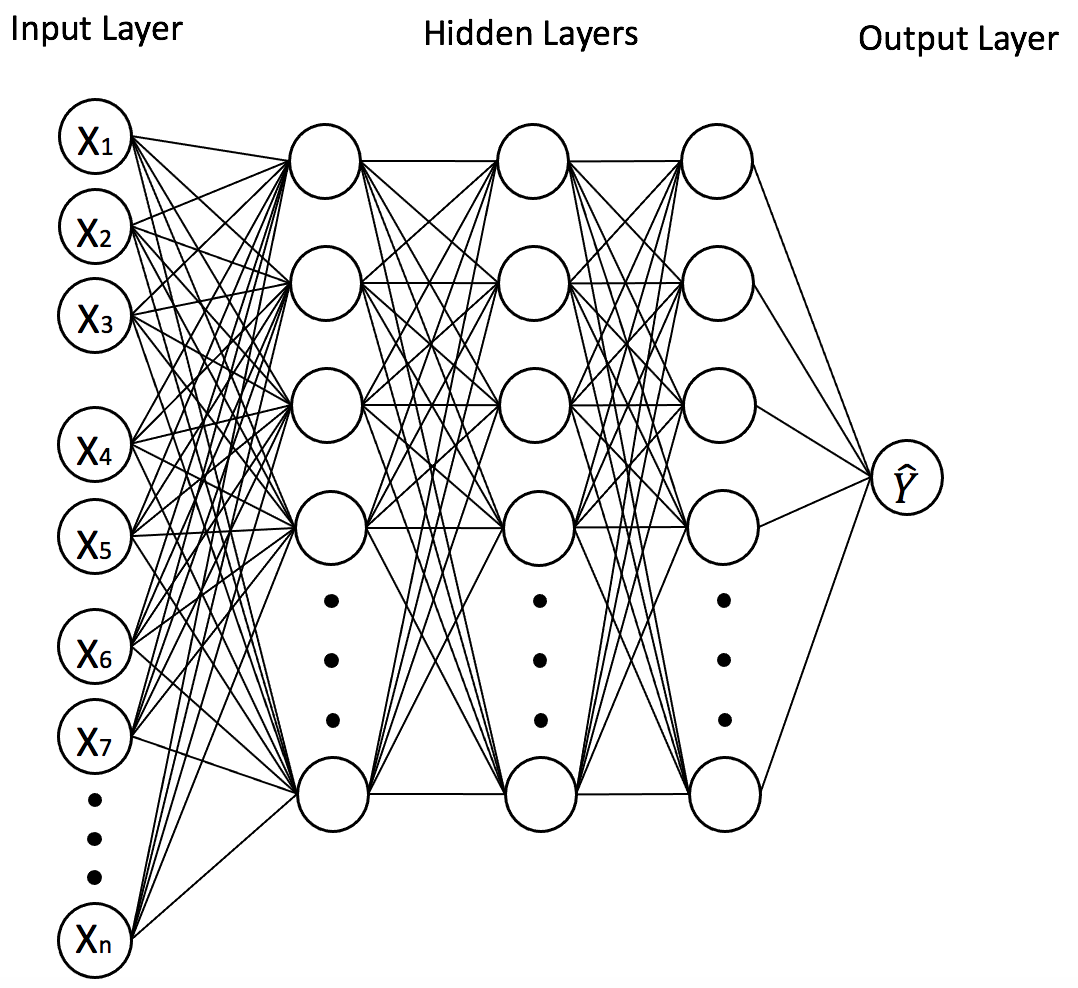
\includegraphics [scale=0.60,angle=360]{figures/neur.png}
\caption{Illustration of a Neural Network}
\label{fig:neur}
\end{figure}

\indent\newline
Figure 2.2 illustrates a traditional neural network, where the nodes represent artificial neurons. These can be compared to the biological neurons of the human brain. The nodes are a graphical representation of numeric values, while the connections can be thought of as the axons in the biological neuron. These connections have different dynamic weights that change as the network trains to learn the patterns within the data. The strength of the connections also changes with an aim for the network to set the right weights, in order to make accurate predictions \cite{opper}. The layers of the neural network can be divided into an input layer, hidden layers and an output layer. The input layer is where the network receives the input data \textit{x}, which consist of features considered to have an explanatory effect on the dependent variable. Each \textit{x} is an entire vector where an input neuron represents one element in the vector. The hidden layers are where mathematical operations are performed in order for the neural network to obtain a prediction vector \textit{y}. Lastly, the output layer is where the network's predictions are being made. An output neuron consists of the value of the prediction, which is a vector \textit{y}. The values presented in this layer could either be a probability value between 0 and 1 (classification) or an infinite value predicting a desired target value (regression) \cite{opper}. 

\indent\newline 
\begin{figure}[H]
\centering
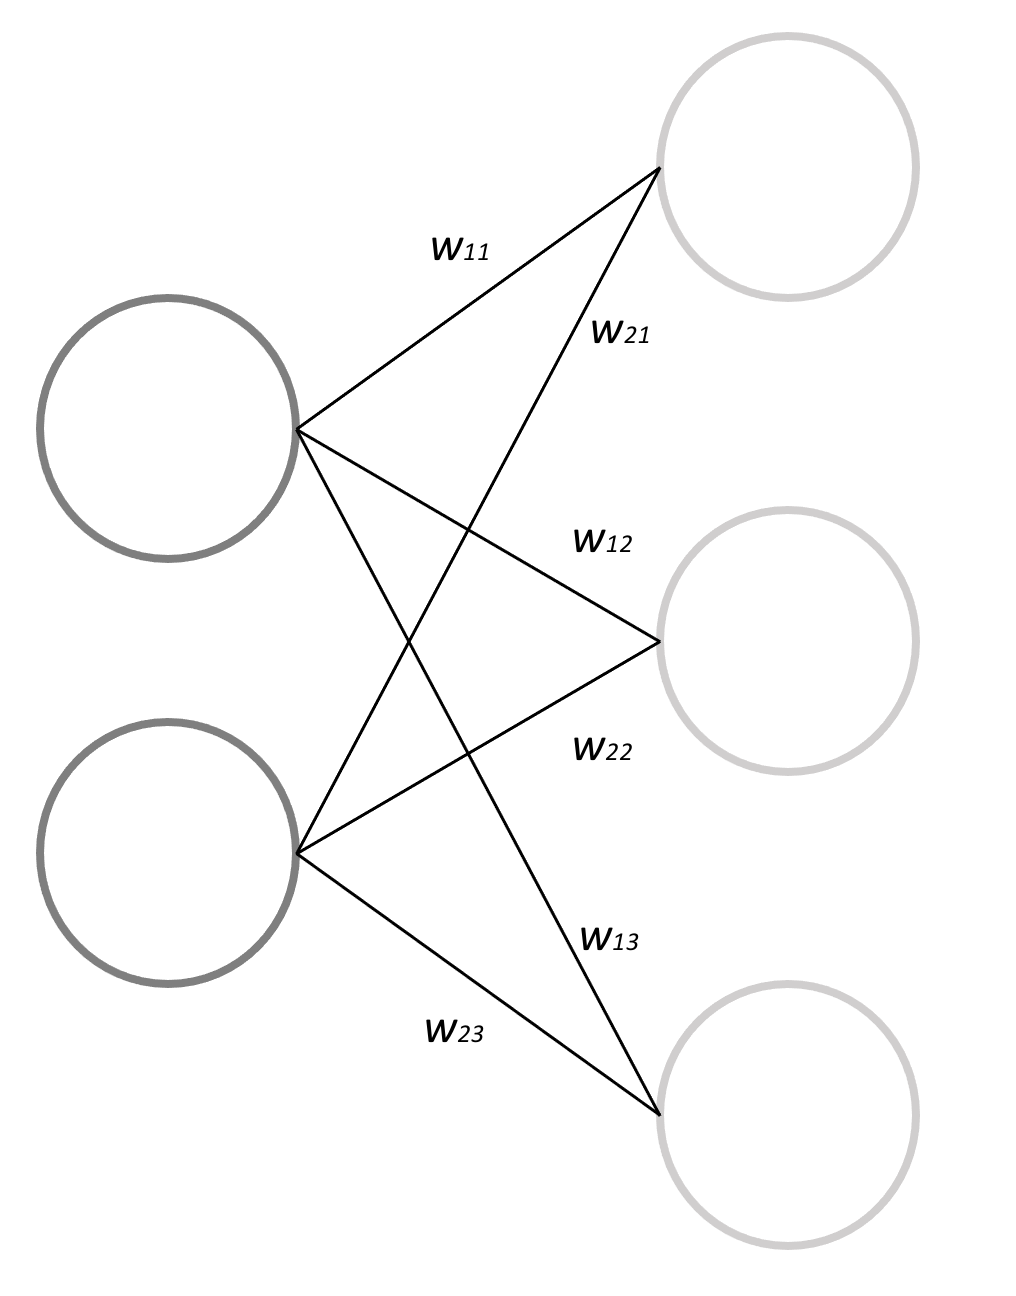
\includegraphics [scale=0.40,angle=360]{figures/weights.png}
\caption{Weights in a Neural Network}
\label{fig:weights}
\end{figure}

\indent\newline 
Figure 2.3 shows an example of a simple neural network with an input layer consisting of two neurons and an output layer with 3 neurons. Each connection between two neurons is represented by a weight w, where each weight has indices. The first number of indices tells us the number of neurons from the connection's origin, while the second value tells us the number of neurons in the layer where the connection leads. The weights between the layers of a neural network can be illustrated through a weight matrix, which is shown below. 
\indent\newline 
\begin{center}
\textit{W} = \begin{pmatrix}
w_{11} & w_{12} & w_{13}\\
w_{21} & w_{22} & w_{23}
\end{pmatrix}
\end{center}

\indent\newline 
The number of entries in a weight matrix corresponds to the number of connections between neurons. This means that the dimensions of the matrix is determined by the layers' size and their connections. The weight matrix above has two rows, since there are two neurons in the input layer and three columns because of the three neurons in the output layer \cite{opper}.

\subsection{The Learning Process}
Having established the basic concepts and structures of a neural network, this section will look at how the network learns. Forward propagation consists of the step where the neural network performs a prediction vector based on an input feature vector \textit{x}. The prediction vector will here be termed as \textit{h}. The dot product of the weight matrix \textit{W} (explained in the previous section) and the input vector \textit{x} is then computed, which gives the vector \textit{z}.

\indent\newline 
\overrightarrow{x}^{T} \cdot W = \begin{pmatrix} x_{1}, & x_{2}
\end{pmatrix} \cdot \begin{pmatrix}
w_{11} & w_{12} & w_{13}\\
w_{21} & w_{22} & w_{23}
\end{pmatrix}}
  
\indent\newline 
= \begin{pmatrix}
x_{1}w_{11}+x_{2}w_{21}, & x_{1}w_{12}+x_{2}w_{22}, & x_{1}w_{13}+x_{2}w_{23}
\end{pmatrix}

\indent\newline 
= \begin{pmatrix}
z_{1}, & z_{2}, & z_{3}
\end{pmatrix} = \overrightarrow{z}, \overrightarrow{h} = \sigma(\overrightarrow{z})

\indent\newline 
In order to obtain the prediction vector \textit{h}, one of three non-linear activation functions is applied to the dot product vector \textit{z}. The three activation functions can be either tanh, sigmoid or ReLu, which enables a non-linear mapping from \textit{z} to \textit{h}. This allows the network to understand non-linear data through the linear combination value of the weights and neurons and the non-linear activation function.

\indent\newline 
The last part of the learning process of the neural network, and the last step in forward propagation, consists of computing a loss function \textit{L}. This phase consists of comparing the prediction vector \textit{y} with the ground truth $\widehat{y}$. The ground truth label represents the actual values, where the difference between the values of $\widehat{y}$ and the predicted values \textit{y} are computed in order to measure the network's accuracy. Minimizing the loss function \textit{L} enables the network to learn and adjust the weights accordingly, as the distance between \textit{y} and $\widehat{y}$ is revealed to the  network. In other words, the network is able to learn how the parameters $\theta$ contribute to the loss function and how it should change these parameters in order to decrease the distance between $\widehat{y}$ and \textit{y}.

\indent\newline 
Two of the most common loss functions implemented in deep learning are the mean squared error loss and the cross-entropy loss. 

\indent\newline 
\textbf{Mean squared error loss:}

\indent\newline 
L(\theta) = \frac{1}{N} \sum_{i=0}^{N} (y_{i} - \widehat{y}_{i})^{2}

\indent\newline 
Where,
\indent\newline 
$y_{i}$ = entries in the prediction vector $\overrightarrow{y}$
\indent\newline 
$\widehat{y_{i}}$ = entries in the ground truth label $\widehat{\overrightarrow{y}}$

\indent\newline 
\textbf{Cross-Entropy Loss:}

\indent\newline 
L(\theta) = - \sum_{i=0}^{N} \widehat{y_{i}} \cdot log(y_{i})

\indent\newline 
Where,
\indent\newline 
$y_{i}$ = entries in the prediction vector $\overrightarrow{y}$
\indent\newline 
$\widehat{y_{i}}$ = entries in the ground truth label $\widehat{\overrightarrow{y}}$

\indent\newline 
\cite{opper}.

\indent\newline 
Minimizing the loss function is solved mathematically by the method termed gradient descent. The method involves taking the derivative of the loss function where each gradient descent step enables the network to get closer in optimizing the weights, and ultimately make satisfying predictions. A simplified example would be a neural network with one input neuron, one output neuron and one connecting weight value, where the network first performs an inaccurate prediction based on a certain weight value. To improve the accuracy a loss function needs to be chosen (in this case a quadratic loss function) where the gradient descent method will update the weight with a more correct value. 

\indent\newline 
\begin{figure}[H]
\centering
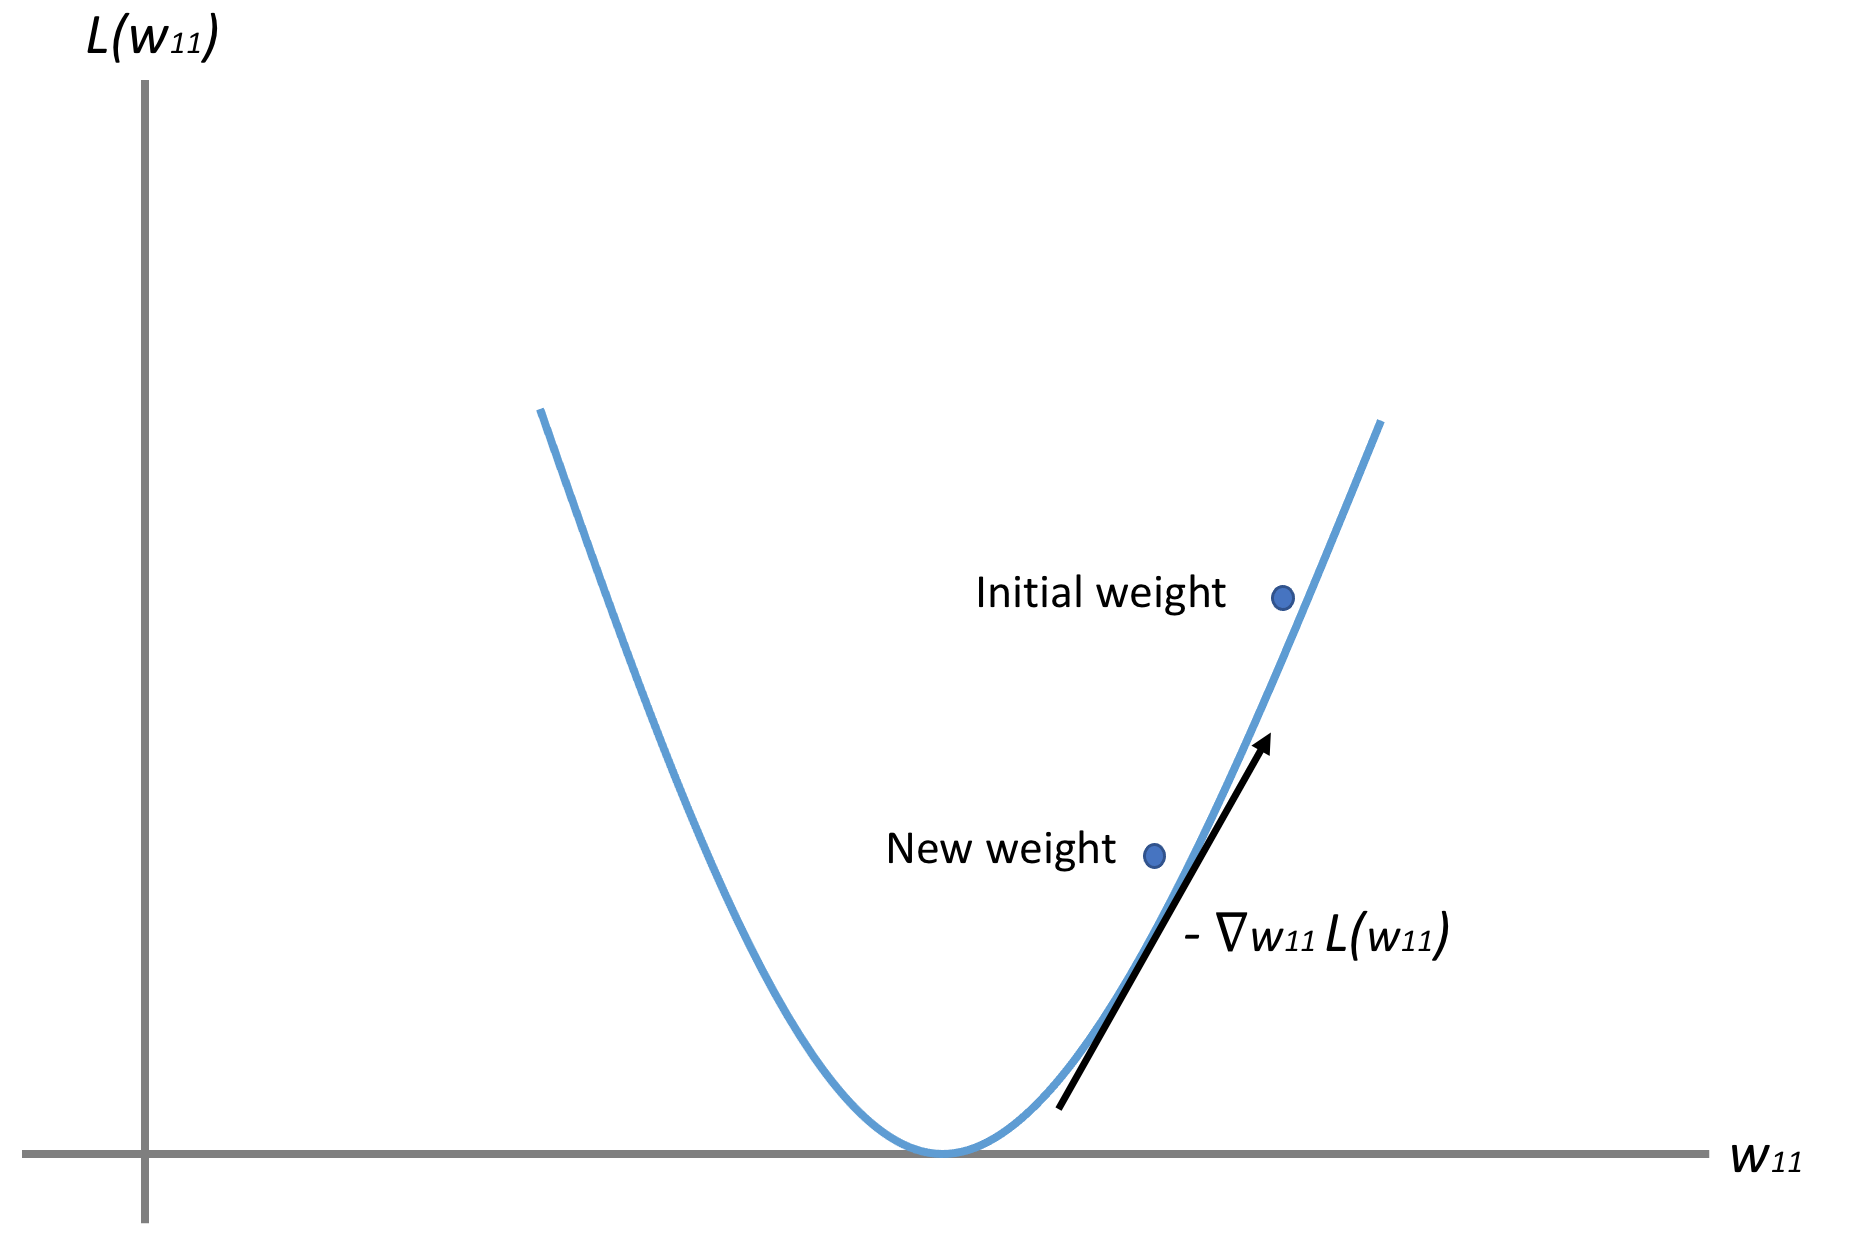
\includegraphics [scale=0.40,angle=360]{figures/gradient.png}
\caption{Gradient Descent}
\label{fig:gradient}
\end{figure}

\indent\newline 
The x-axis in figure 2.4 is the value of the weight, while the y-axis is the difference between the ground truth and the prediction, and essentially the network parameters (the value of the loss function). Using a quadratic loss function means that there is only a global minimum and not a local minimum. The global minimum represents the value of the weight that enables the network to make an accurate prediction, and is shown in the figure as the point where the loss function is equal to zero. In the fictive example shown in the figure, the initial prediction and weight value is relatively inaccurate. To improve the accuracy of the prediction, the next step involves updating the weight parameter until it reaches an optimized value for the weight. This is carried out by taking the derivative of the loss function with respect to the weight \textit{w}.

\indent\newline
\nabla_{w11} L(w_{11}) = \frac{\partial L(w_{11})}{\partial w_{11})}

\indent\newline
The equation computes the tangent (slope) of the loss function for the point of where the initial weight lies. The figure shows that the tangent of the loss function would be positive, which would correspond to the network updating the weights to a higher loss value and making even more inaccurate predictions. However, this can be solved by multiplying the gradient by minus one to get the opposite direction of the gradient.  

\indent\newline
w_{11_{new}} = w_{11_{old}} - \epsilon \cdot \nabla_{w11} L(w_{11})

\indent\newline
The equation above shows a step of the gradient descent where the network updates the value of the weight to make a more accurate prediction. In the equation, epsilon is implemented as the network’s learning rate and represents how quickly the parameters are updated. This method of updating the parameters continues until the loss function reaches a point of global minimum, which represents the optimal weight value for the network to perform accurate predictions \cite{opper}.  

\subsection{LSTM Network}
Unlike feed forward neural networks (FNNs) explained in the previous section, long short-term memory networks (LSTMs) is a type of recurrent neural network (RNN). Comparing RNNs with FNNs, RNNs resemble a more accurate representation of the workings of a biological neural network. The human brain has the ability to retain previous learnt information while receiving new information, which can either change a perceived outcome or it can remain unchanged. The same logic applies to RNNs, where loops within the networks are utilized to incorporate past information in the final output \cite{adu}. 

\indent\newline 
\begin{figure}[H]
\centering
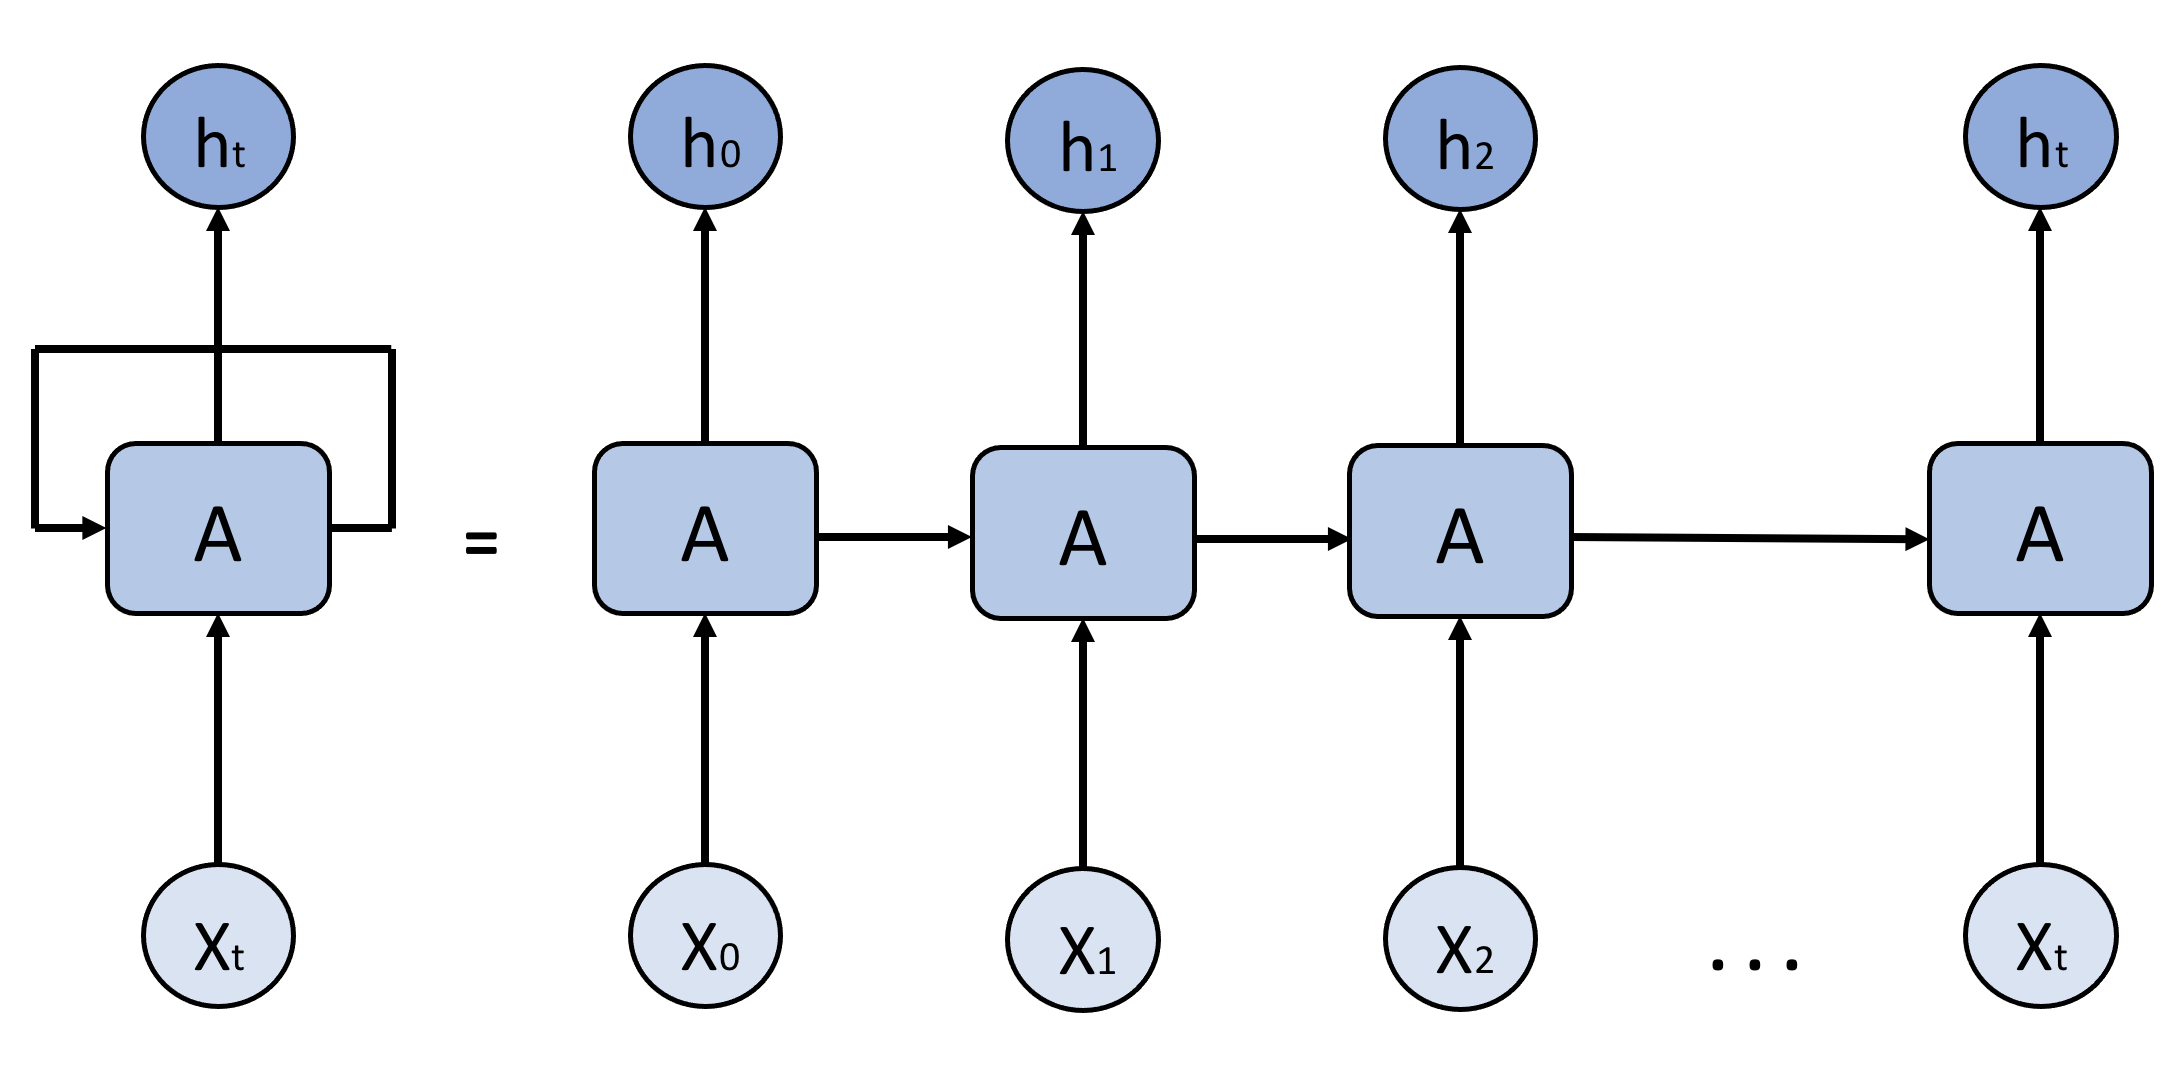
\includegraphics [scale=0.32,angle=360]{figures/rnn.png}
\caption{Structure of a Simple RNN}
\label{fig:rnn}
\end{figure}

\indent\newline 
Figure 2.5 illustrates a simple RNN where \textit{A} represents a piece of neural network (repeating module), $X_{t}$ is some input, $h_{t}$ an output value, while the loop allows the network to pass information from each step to the next. The right side of the figure illustrates a recurrent neural network if it had been unrolled, and demonstrates a chain-like characteristic useful for data consisting of sequences and lists \cite{olah}.    

\indent\newline 
A limitation with simple RNNs is their ability to retain previous learnt information over longer periods of time. Their short-term memory is connected to the vanishing gradient problem \cite{phi}. During backpropagation, these simple RNNs' gradients shrink as they back propagate through time and their values become extremely small. This applies normally to the earlier layers when the update values become so small that the layers stop learning. This can make the RNNs forget what they have previously seen. In relation to predicting stock returns, LSTM is a type of RNN which can cope with this problem since financial time series requires predictive models to train on large data sets, stretching over a long period of time. 
\indent\newline 
\begin{figure}[H]
\centering
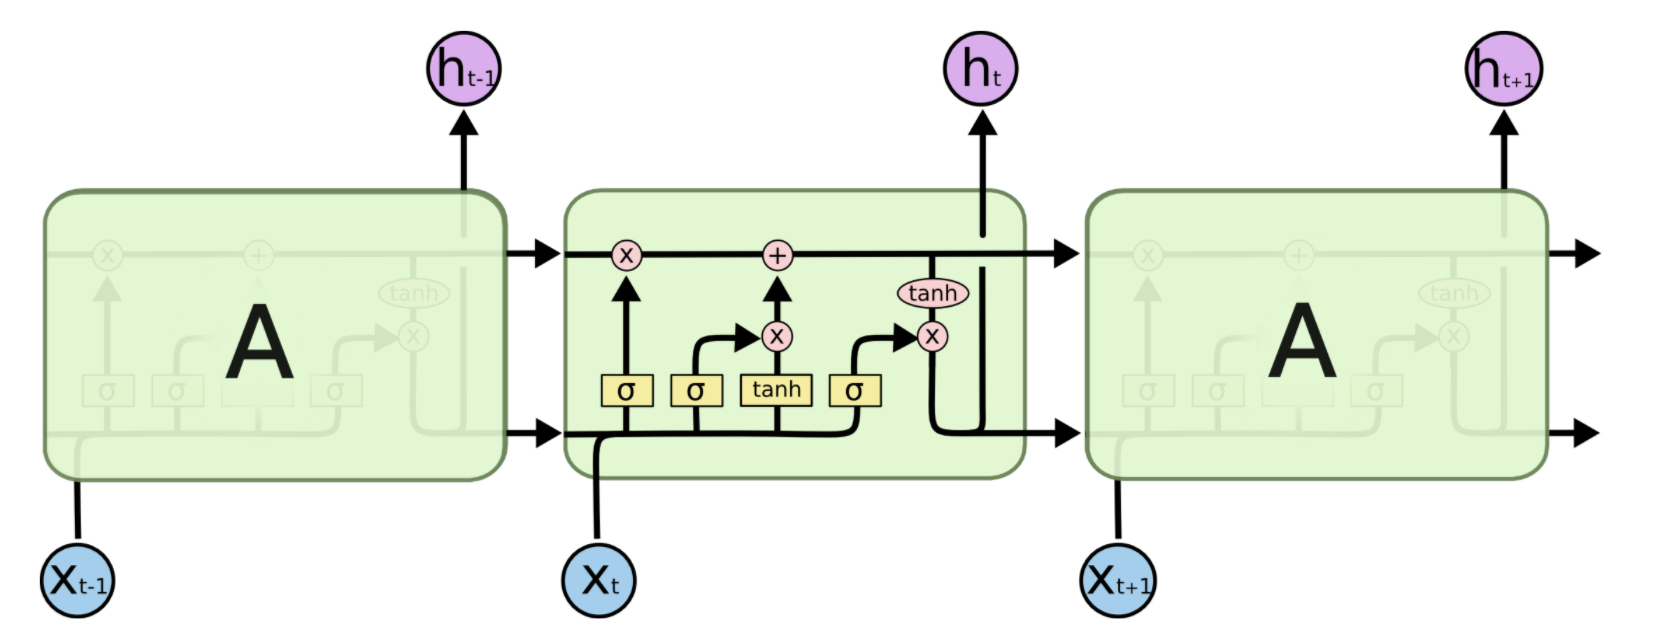
\includegraphics [scale=0.40,angle=360]{figures/lstm.png}
\caption{Structure of a LSTM-Network (source: \cite{olah})}
\label{fig:lstm}
\end{figure}

\indent\newline 
Figure 2.6 illustrates the recurrent system of an LSTM. The yellow boxes represent learned network layers, the pink circles are pointwise operations, while each line visualize how the LSTM carries entire vectors. Merging lines depict concatenation and lines that fork is a representation of copied contents going to other locations \cite{olah}. 

\indent\newline 
\begin{figure}[H]
\centering
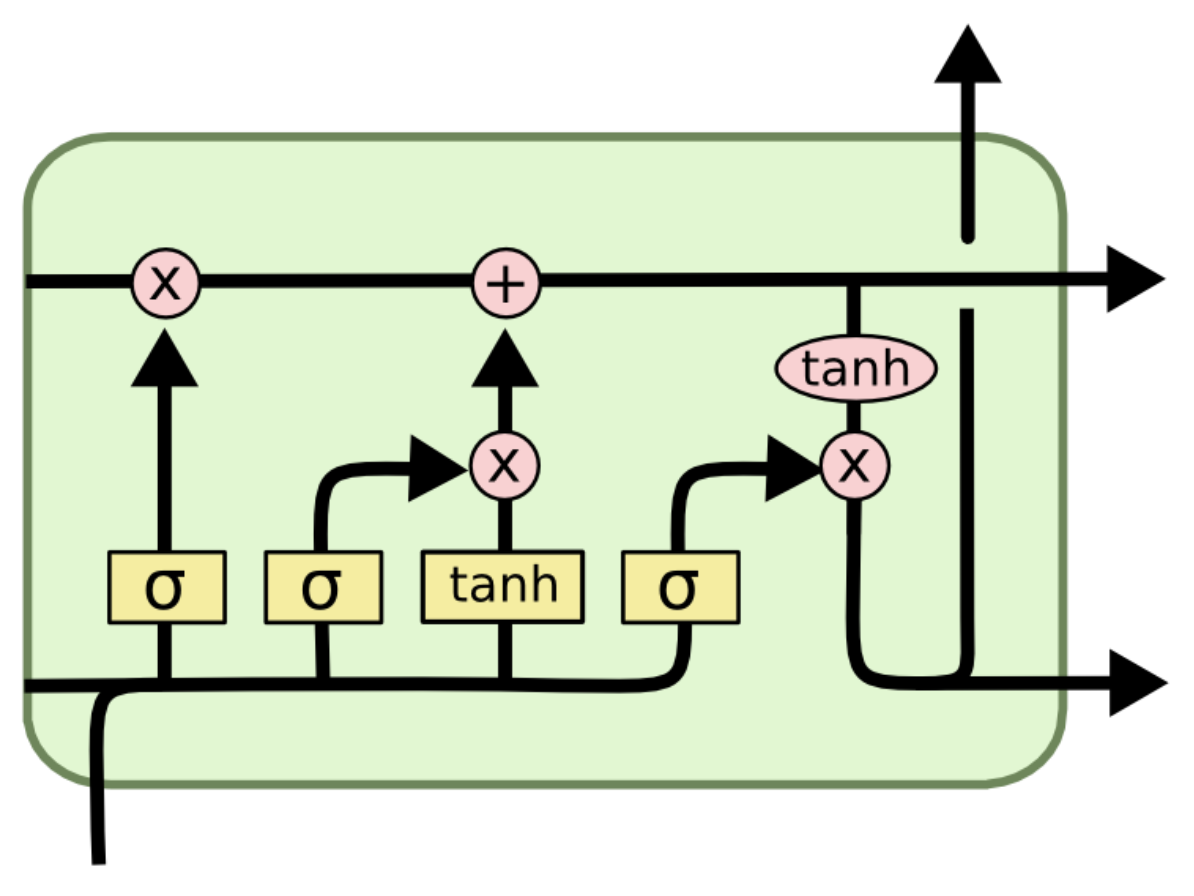
\includegraphics [scale=0.40,angle=360]{figures/module.png}
\caption{The Repeating Module (source: \cite{olah})}
\label{fig:module}
\end{figure}

\indent\newline 
One of the main differences between a simple RNN and an LSTM is the repeating module. A standard RNN only has a single neural network layer, while an LSTM has four interacting neural network layers. The horizontal line running through figure 2.7 illustrates the cell state $C_{t}$. This represents the flow of information through the network chain. In order for the LSTM to regulate the information being passed through, three different types of gates are used. The gates are made up of a neural network layer and a pointwise multiplication operation, and consist of a forget gate $f_{t}$, an input gate $i_{t}$, and an output gate $o_{t}$ \cite{olah}. The forget gate is a sigmoid layer that decides which parts of the information to forget. $f_{t}$ outputs a value between 1 and 0 for each number in the cell state $C_{t-1}$ by evaluating $h_{t-1}$ and $x_{t}$, where a value of 1 means keeping all of the information and a value of 0 means forgetting all of the information:

\indent\newline 
$f_{t}$ = \sigma(W_{f} \cdot[h_{t-1},x_{t}] + b_{f})

\indent\newline 
The next two parts of the LSTM decide what new information to be stored in the cell state. The first part consists of an input gate where a sigmoid layer decides which values to update\cite{olah}. Then, a vector of new candidate values Ct are created by a tahn layer, which represents potential values to be added to the state:

\indent\newline 
$i_{t}$ = \sigma(W_{f} \cdot[h_{t-1},x_{t}] + b_{i})

\indent\newline 
$\tilde{C_{t}}$ = tanh(W_{C} \cdot[h_{t-1},x_{t}] + b_{C})

\indent\newline 
Having determined the information to forget and keep from memory, how much information that will be added to the memory, and candidate values to be added, the next step involves updating the cell state:

\indent\newline 
C_{t} = f_{t} \ast C_{t-1} + i_{t} \ast \tilde{C_{t}}

\indent\newline 
The old state is multiplied with the forget gate layer $f_{t}$, while the new, scaled candidate values $i_{t}*\tilde{C_{t}}$ are added. The final step is for the LSTM to decide on the output. A sigmoid layer determines which parts of the cell state to output, before the cell state runs through a tanh layer in order to transform the values into values between -1 and 1 \cite{olah}: 

\indent\newline 
$o_{t}$ = \sigma(W_{o} \cdot[h_{t-1},x_{t}] + b_{o})

\indent\newline 
$h_{t}$ = o_{t} * tanh(C_{t})

\subsection{GRU}
The Gated Recurrent Unit (GRU) is a variation of an RNN and an LSTM network. Compared to LSTM, the GRU is a more simple model where the forget and input gates are combined into an update gate, as well as having merged the cell state and hidden state \cite{olah}. 

\indent\newline 
\begin{figure}[H]
\centering
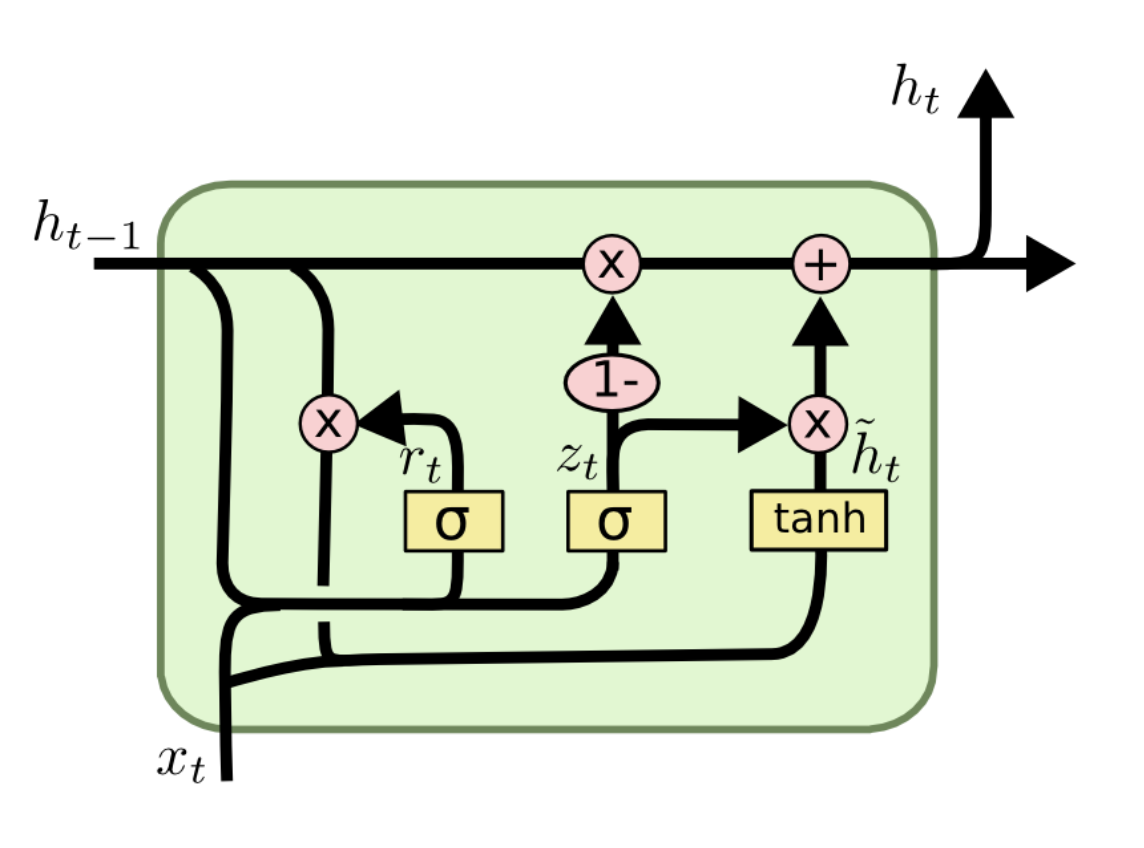
\includegraphics [scale=0.40,angle=360]{figures/gru.png}
\caption{Structure of a Gated Recurrent unit (source: \cite{olah})}
\label{fig:gru}
\end{figure}

\indent\newline 
In the update gate, $x_{t}$ is plugged into the network unit and multiplied by the weight $W_{z}$. $h_{t-1}$ holds previous information and is also multiplied by its weight $U_{z}$. Further, a sigmoid activation transforms the result into a value between 0 and 1 \cite{kosta}:

\indent\newline 
$z_{t}$ = \sigma(W_{z} x_{t} + U_{z} h_{t-1})

\indent\newline 
Similar to the LSTM, in this step the GRU determines which parts of the past information to pass along in the structure, where a value of 1 means copying all of the past information and a value of 0 means keeping none of the information. Further, the reset gate is used to determine which parts of the information to forget. The same logic of the update gate applies to the reset gate:

\indent\newline 
$r_{t}$ = \sigma(W_{r} x_{t} + U_{r} h_{t-1})

\indent\newline 
The next step of the process is introducing a memory content, in order for the network to be able to utilize the reset gate to store relevant information from the past \cite{kosta}:

\indent\newline 
$\tilde{h_{t}}$ = tanh(W_{x_{t}} + r_{t} * U_{h-1})

\indent\newline 
The equation allows the model to determine what to remove from previous learned information, before applying the nonlinear activation function tanh, to transform the results into values between -1 and 1. The last step of the GRU is using the update gate to decide what information to collect from the current memory content $\tilde{h_{t}}$ and the previous steps $h_{t-1}$ \cite{kosta}. In order to do so, the model calculates $h_{t}$, which is a vector with information for the current unit and with a function of passing the information down in the network structure:

\indent\newline 
$h_{t}$ = z_{t} * h_{t-1} + (1 - z_{t}) * \tilde{h_{t}}

\subsection{CNN}
Convolutional neural networks (CNNs) is a type of feedforward neural network commonly used for image recognition and object classification. The structure of a CNN can be compared to the neurons in the human brain, where individual neurons respond to stimuli in several Receptive Fields (parts of the visual field) that overlap each other to cover the entire visual area \cite{saha}.   

\indent\newline 
\begin{figure}[H]
\centering
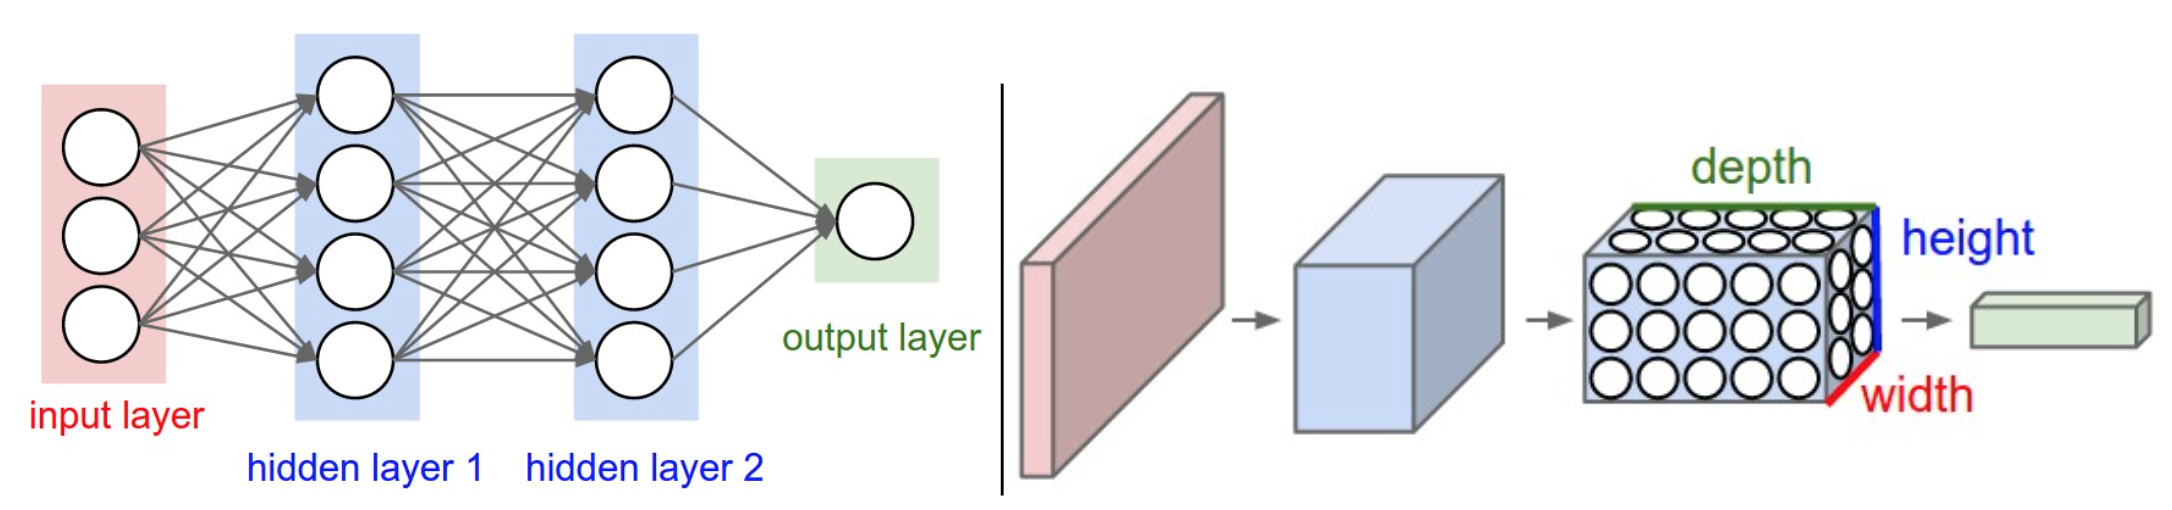
\includegraphics [scale=0.34,angle=360]{figures/cnn.png}
\caption{Structure of a CNN (source: \cite{zakka})}
\label{fig:cnn}
\end{figure}

\indent\newline 
The architecture of a CNN differs from standard neural networks in terms of making an assumption of input being images, which reduces the amount of parameters in the model. Figure 2.9 displays the difference between them where the neurons in a CNN are arranged in three dimensions, which consist of width, height and depth (illustrated in the third layer). The third dimension of depth refers only to an activation volume and not the depth of an entire neural network \cite{zakka}. In addition to having fully connected layers, as in standard neural networks, the CNN uses convolutional layers and pooling layers to reduce spatial size of the convolved feature. 

\indent\newline 
In the convolution layer a kernel K performs a matrix multiplication operation of K and P (the part of the image the kernel hovers over) equal to the number of stride lengths. The process is repeated until the image is traversed \cite{saha}. A CNN can have multiple convolutional layers, where the first one uses the input image to extract low-level features, while the last ones enables the model to adapt to the high-level features. Further, pooling layers reduce the amount of computational power needed to process the data, by reducing the spatial size of the convolved feature and by reducing dimensionality. There are two types of pooling, namely max pooling and average pooling, which consist of the model returning either the maximum value from the portion of the image covered by the kernel, or the average of all the values\cite{saha}. This is useful for extracting dominant features, as well as suppressing noisy activations. The last steps of the CNN-architecture consist of flattening the final output, before feeding it into a neural network (fully connected layer) to perform the classification.   

\section{Backtesting}
Developing new trading strategies can be a difficult task, and especially for investors to gain the confidence to implement the strategies in real-life trading. Backtesting, or systems testing, is an important method used by brokers and professional investors to test new strategies in a simulated environment. Backtesting reconstructs a trading scheme on historical data that would have occurred by using a particular trading strategy. An assumption within backtesting is that if a trading strategy has performed well in the past, it will also probably perform well in the future. Vice versa, if a trading strategy has performed poorly in the past, there is a good chance it will perform poorly in the future as well \cite{ni}.  To evaluate the performance of a trading strategy, several statistics and metrics can be used. This includes net profit or loss, volatility measures, average gain or loss, the percentage of capital exposed to the market, win-loss ratios, annualized return, and risk-adjusted return \cite{kuepper}. 

\indent\newline
Backtesting trading strategies comes with several potential pitfalls that can cause a seemingly successful strategy to fail when applying it to real-life trading: 

\begin{itemize}
\item \textbf{Market trend:} The time period and broad market trend are important factors to consider when conducting backtesting. If a strategy is backtested on a time period characterized by a consecutive bull market, the chances are the strategy will not perform well in a bear market. Backtesting should therefore be carried out on historical data with market conditions that include both a positive and negative market sentiment. 
\item \textbf{Universe:} Backtesting should also consider the universe the system is tested in. Developing a trading strategy targeted towards small cap stocks, and backtesting it in a universe of large cap stocks, will probably not translate into developing a successful strategy. It is therefore important to be aware of the limitations of a given strategy, while making sure the backtesting complies with these limitations.
\item \textbf{Volatility:} Traders who have leveraged accounts should focus their attention on volatility. Leveraged investors are subjected to margin calls, which occurs when an investor’s account value drops below the broker’s threshold. It is recommended for these investors to include volatility measures where the backtesting results in low volatility to minimize risk.   
\item \textbf{Risk:} Risk: A common mistake when backtesting is only focusing on annualized returns without taking into account the change in risk. Annualized returns is often used as a metric to compare the performance of a strategy against other suitable benchmark strategies. Risk-adjusted returns is an alternative metric which should be implemented in backtesting, in order to be certain that a potential trading strategy actually outperforms other benchmark strategies with an equal (or lower) level of risk.     
\item \textbf{Storytelling:} In situations where an investor has worked hard to develop a new trading strategy it is not uncommon to be biased. Since backtesting involves testing strategies on historical data (ex-post), it is possible that the investor justifies certain patterns and results with rationality that skews the results in the investor’s favour. This could potentially lead to applying strategies that underperform against other more well-established trading strategies. 
\item \textbf{Transaction costs:}  Simulating the transaction costs of each trade being made in backtesting is difficult because it would require the trades to be actually carried out under the       
\item \textbf{Transaction costs:} Simulating the transaction costs of each trade being made in backtesting is difficult because it would require the trades to be actually carried out in the real world. The bid-ask spread varies greatly between individual stocks, which can be hard to simulate correctly.        
\item \textbf{Over-optimization:} This is a condition where performance results are overfitted to the past. There is no guarantee the past will repeat itself, which means that fine-tuning parameters too much to the past can cause a strategy to fail in the present and future.    
\end{itemize}

\indent\newline   
Investors should keep these potential pitfalls in mind when backtesting a new trading strategy. Even if these frequent backtesting errors are avoided, it does not mean a good performance backtest will result in successful performance in the future. There will always be a chance of selection bias and a chance of history not repeating itself.   

\section{Transaction Costs}
As mentioned in the previous section, accurately simulating transaction costs is a common error when developing a trading strategy. To be able to accurately simulate the transaction cost for each given trade, it would require traveling back in time and actually executing each trade. To best cope with this problem, an investor needs to be aware of the different elements of transaction costs and how these elements affect the overall trading performance. The elements consist of:

\begin{itemize}
\item \textbf{Explicit transaction costs:} Broker commission and securities lending.
\item \textbf{Implicit transaction costs:} Arrival cost and implementation shortfall.
\end{itemize}  
\cite{morgan}

\indent\newline   
Explicit transaction costs can be decomposed into broker commissions and securities lending. Broker commissions is a fee an investor is required to pay in order to have a brokerage company facilitate a transaction. These fees vary between brokers, but it can have a substantial impact on returns, especially when a strategy requires frequent trading. Securities lending is directed at short selling activities. Short selling is when an investor borrows another investor's shares and sells these shares in the market, where the purpose is to buy back the same amount of shares at a later point at a lower price, before delivering the stocks back to the investor. Short sellers pay a borrowing fee to the investor who agreed to lend out the shares. 

\indent\newline   
Implicit transaction costs can be decomposed into arrival cost and implementation shortfall. Arrival cost is the difference between the arrival price and the execution price. The arrival price is the given price an asset is valued at the moment right before an order, while the execution price is the actual traded price \cite{morgan}. Implementation shortfall is the opportunity cost of placing an order below ask and when this order does not get executed. Placing an order below ask might lead to missing the opportunity of taking a position in a stock, which can affect portfolio composition and returns.This part of trading can be quite difficult, where an investor has to decide whether to avoid implementation shortfall all together by filling the current orders at ask, or placing an order below ask with hopes of getting a better entry price. 

\indent\newline   
A common way of backtesting deep learning trading algorithms is only including direct transactions costs. This underestimates the total transaction costs of a trading strategy, and can result in over-optimistic returns and results from the backtesting. Previous academic papers have usually assumed direct transaction costs of five basis points \cite{krauss}, while research carried out in 2009 on the Oslo Stock Exchange, showed arrival costs of 200 basis points by studying the period between 2000-2008 \cite{ode}. Since implicit transaction costs can potentially have a substantial impact on returns, it is important to include these costs in backtesting as an investor would experience arrival costs in practice.     

\section{Market Capitalization}
The market capitalization of a stock, also frequently mentioned as market cap, is the total market value of a company. It is a measure based on a company's worth in the open market and can be found by multiplying the number of outstanding shares with the last traded share price. How the open market determines a company's market cap is dependent on several factors. A common misconception is that it measures equity. The market evaluation of a company's total value is dependent on several factors. One of the most important factors is the company's ability to generate cash flow. This includes the ability of generating cash flow both in present time and in the future. The market expectation of a company's ability to generate future cash flow is one of the main reasons why a company sometimes can be either overvalued or undervalued. These situations of incorrect short-term evaluation create opportunities of possible profitable trades, which could potentially be exploited by deep learning algorithms.  

\subsection{Large Cap Stocks}
Stocks reviewed as large cap companies are big, solid companies with a stable positive cash flow, often associated with low risk. These stocks are referred to as blue chips, which originates from casinos where blue chips are the most valuable. Blue chips are often associated with solid earnings, low level of debt ratio and frequent cash dividends. Large cap stocks are often preferred by investors seeking a low level of risk, high volume of traded shares, and expectations of small fluctuations (low volatility) in share price. The Oslo Stock Exchange (OSE) is a smaller stock exchange which means that the classification of large cap stocks differ from larger stock exchanges such as S\&P 500, Dow Jones and Nasdaq in the US. These typically classify companies with a market capitalization of minimum 10 billion dollars as large cap stocks, while at the Oslo Stock Exchange this boundary is set to a market cap above 15 billion NOK (approximately 1.8 billion dollars). 

\subsection{Small Cap Stocks}
Companies regarded as small cap stocks are small, young companies, where a stable positive cash flow is not expected until several years down the line. The share prices tend to be more volatile with less liquidity than mature companies.These types of companies are often expected to experience significant growth in future years, which makes them difficult to evaluate. Because a positive net cash flow is not expected before many years, investing in these companies brings increased risk. Small caps are therefore often subject to speculations, where the share price can fluctuate greatly, based on changes in the company outlook and in periods of economic slowdowns. The stock exchanges in the US regard companies with a market cap below 2 billion dollars as small cap stocks, while the Oslo Stock Exchange regards companies with a market cap below 1 billion NOK (approximately 120 million dollars) as small cap stocks.   

\indent\newline   
Comparing historical returns favours investing in small caps stocks over large cap stocks. In the period from 1997 to 2012 the small cap index Russel 2000 had an annual return of 8.6\%, while the S\&P 500 had an annual return of 4.8\% \cite{segal}. On the other hand, the small cap index had one-third higher volatility compared to the S\&P 500. Comparing small cap funds with large cap funds in the period 2003-2013 showed a standard deviation (volatility measure) of 19.28 for small cap funds and 15.54 for large cap funds. A higher volatility translates into higher risk, which can make it difficult for investors, who have a limited number of stocks in their portfolio, to capitalize from investing in small cap stocks.  

\indent\newline   
Even though small cap stocks seem to outperform large cap stocks, they have higher volatility that translates into higher risk. Small cap investing with a portfolio consisting of a limited number of stocks can make it difficult for investors to capitalize from this type of investment strategy. 
